%%%%%%%%%%%%%%%%%%%%%%%%%%%%%%%%%%%%%%%%%%%%%%%%%%%%%%%%%%%%%%%%%%%%%%%%
\chapter{Fundamentals}
%%%%%%%%%%%%%%%%%%%%%%%%%%%%%%%%%%%%%%%%%%%%%%%%%%%%%%%%%%%%%%%%%%%%%%%%

This chapter provides a basic understanding of the underlying methods
and concepts, that were required for this work.

%%%%%%%%%%%%%%%%%%%%%%%%%%%%%%%%%%%%%%%%%%%%%%%%%%%%%%%%%%%%%%%%%%%%%%%%
\section{Grids}
%%%%%%%%%%%%%%%%%%%%%%%%%%%%%%%%%%%%%%%%%%%%%%%%%%%%%%%%%%%%%%%%%%%%%%%%

In computational science, discrete data domains are often represented by
grids. The data itself is mostly saved at specific points of the grid
(nodes), or in regions (cells), enclosed by surrounding nodes and the
respective connections (edges) between them. In more rare cases the
values are saved in the edges or the faces of the cells. The
connectivity of the nodes is given by the topology of the grid and
therefore the shape of the cells. There are three types of grids:
scattered data (Figure~\ref{fig:scattered}), which has no topology,
hence no edges connecting the nodes, structured grids, which have an
implicit topology following the ordering of the nodes, with a fixed
number of nodes per dimension, as well as fixed cell types, and
unstructured grids (Figure~\ref{fig:unstructured}), which only have
irregular topology with varying cell types. For the latter the topology
has to be stored explicitly. Structured grids can further be
distinguished into uniform (Figure~\ref{fig:uniform}), rectilinear
(Figure~\ref{fig:rectilinear}) and curvilinear structured grids
(Figure~\ref{fig:curvilinear}). The nodes in uniform grids are
equidistant for every dimension, whereas rectilinear grids may have
irregular spacings along either axis and curvilinear grids may have
irregular spacings between each grid node. This work focuses on uniform
structured grids as it makes it easier to compare multiple grids at
specific points in the domain. Due to the structured grids, we have a
fixed number of nodes along a dimension, which determine the resolution
of this axis.

\begin{figure}
  \begin{subfigure}[b]{0.19\textwidth}
    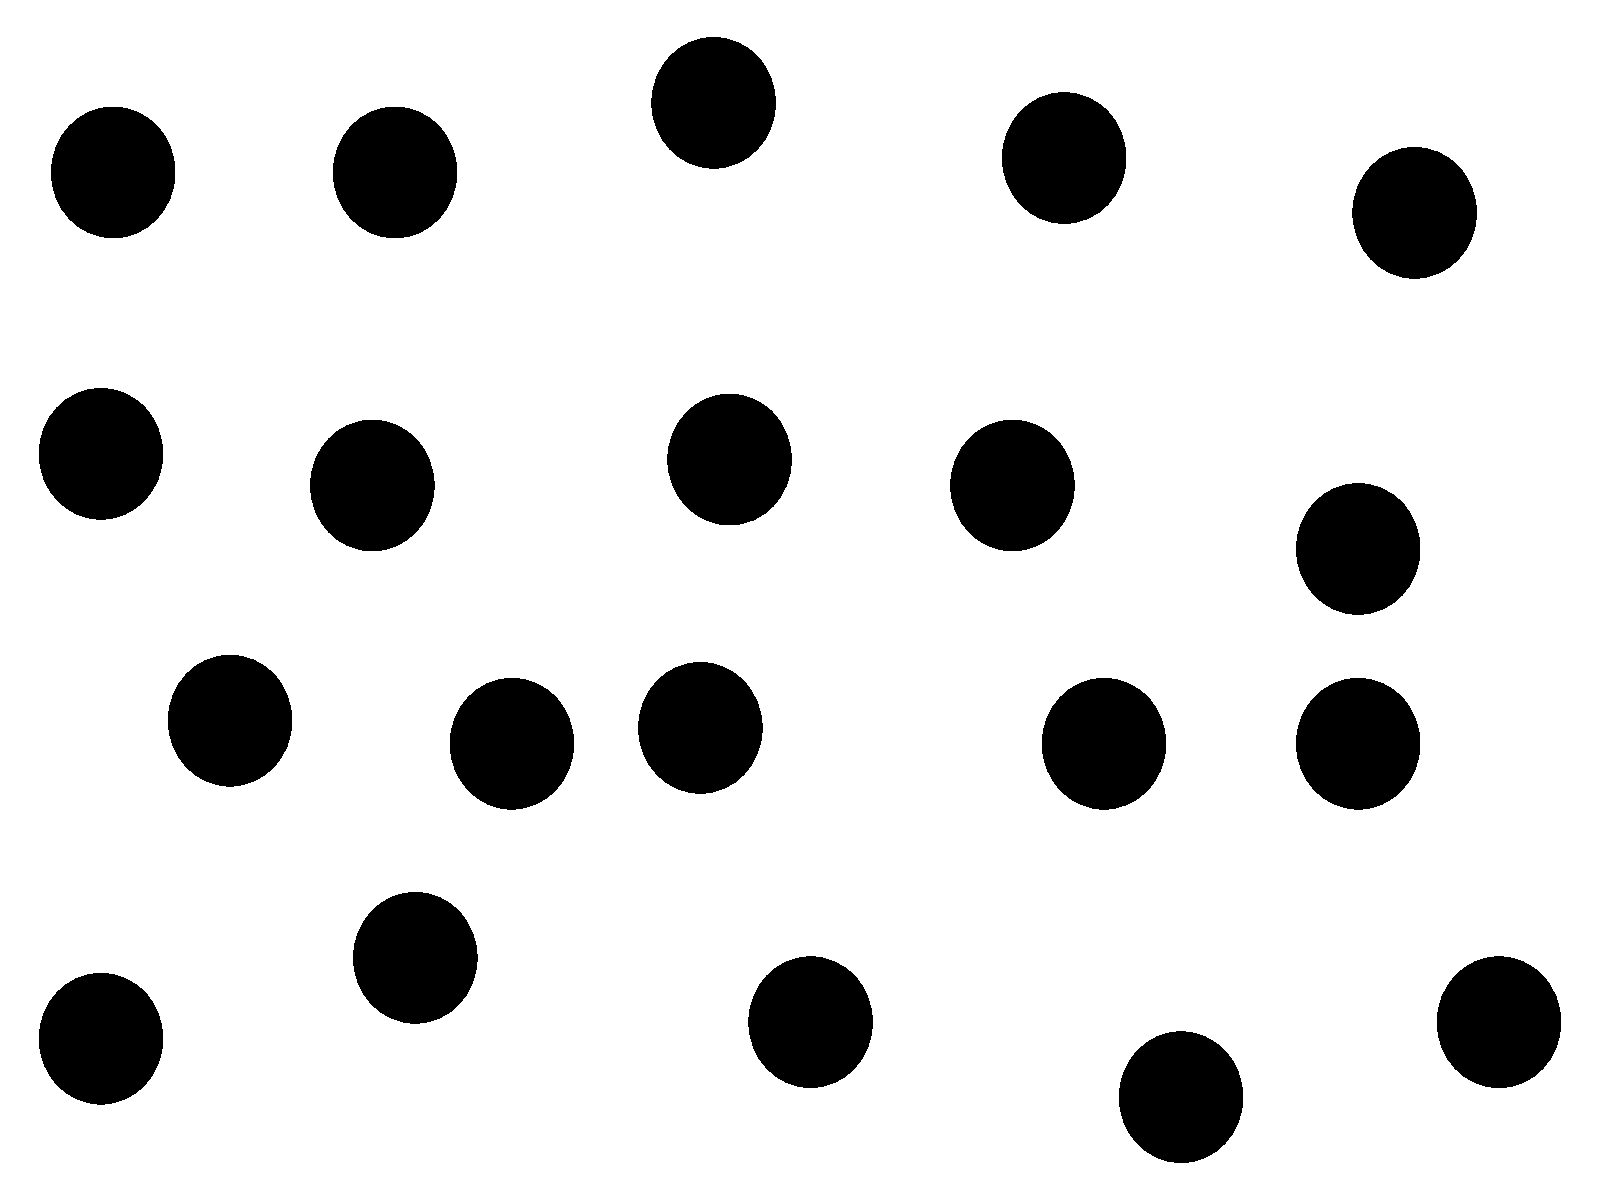
\includegraphics[width=\textwidth]{Images/scattered.pdf}
    \caption{scattered}
    \label{fig:scattered}
  \end{subfigure}
  \begin{subfigure}[b]{0.2\textwidth}
    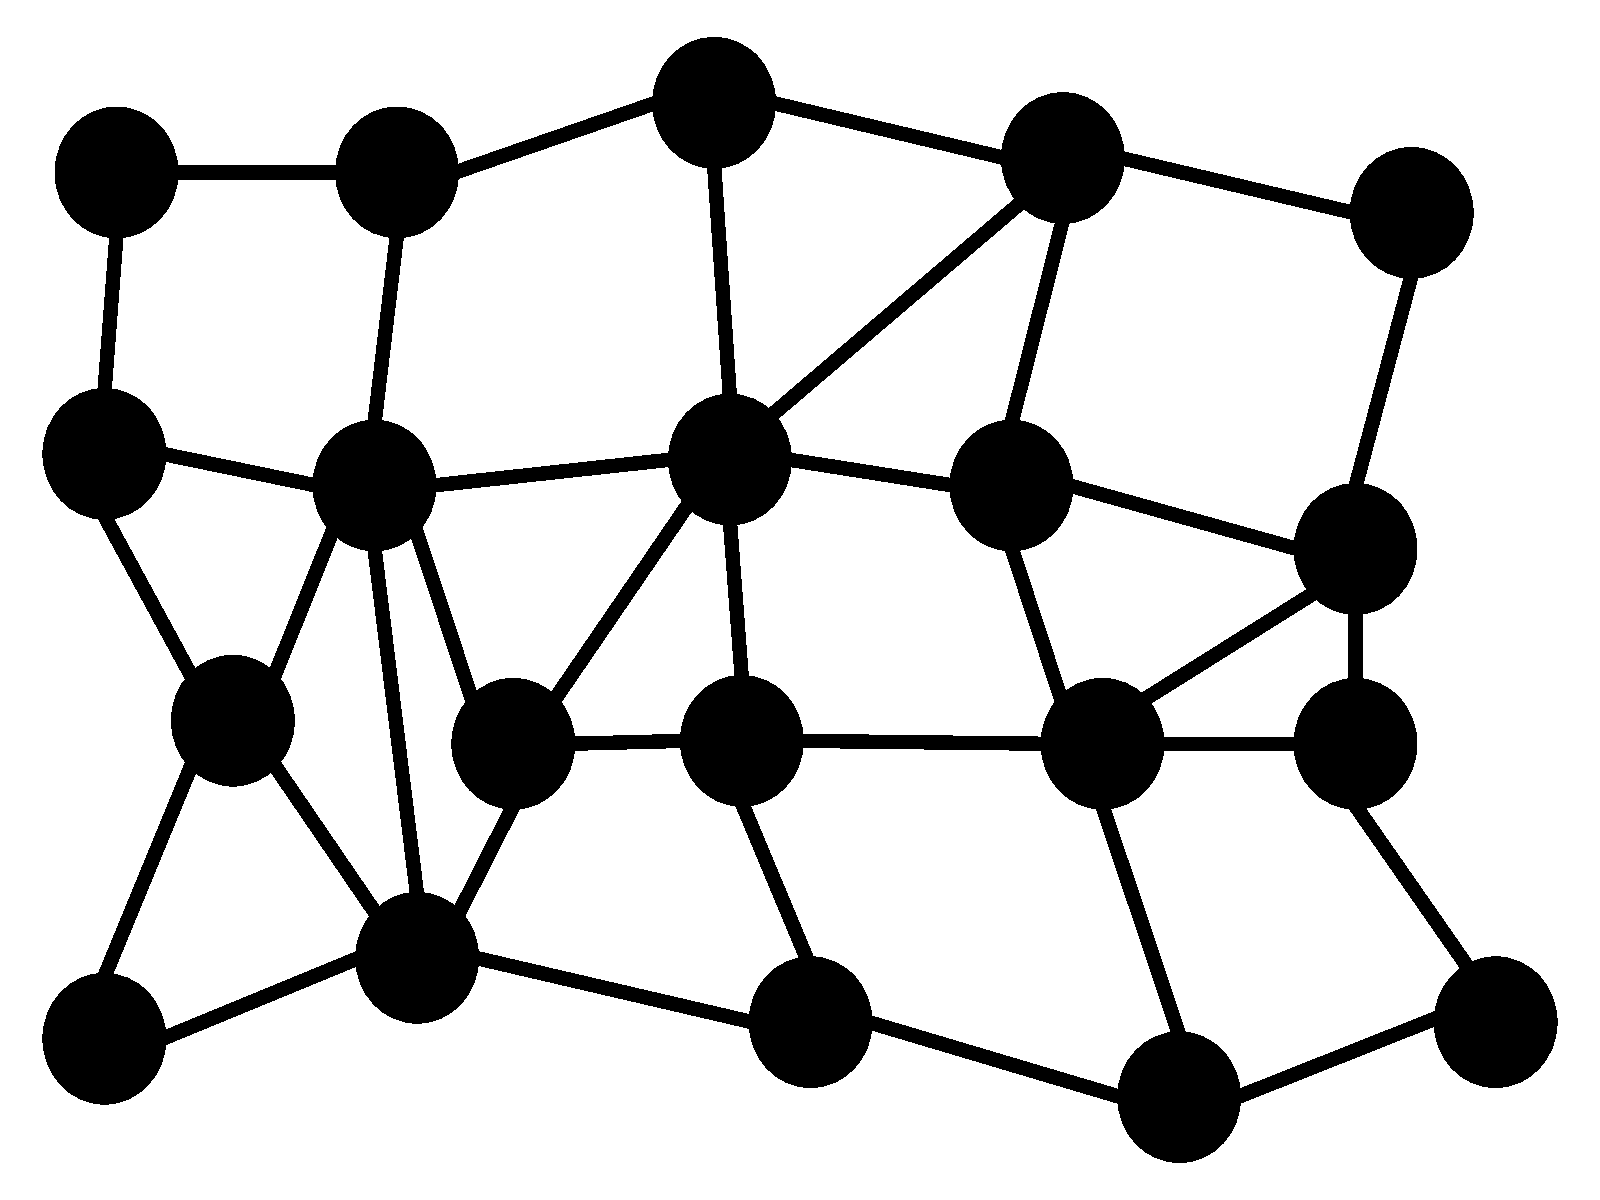
\includegraphics[width=\textwidth]{Images/unstructured.pdf}
    \caption{unstructured}
    \label{fig:unstructured}
  \end{subfigure}
  \begin{subfigure}[b]{0.2\textwidth}
    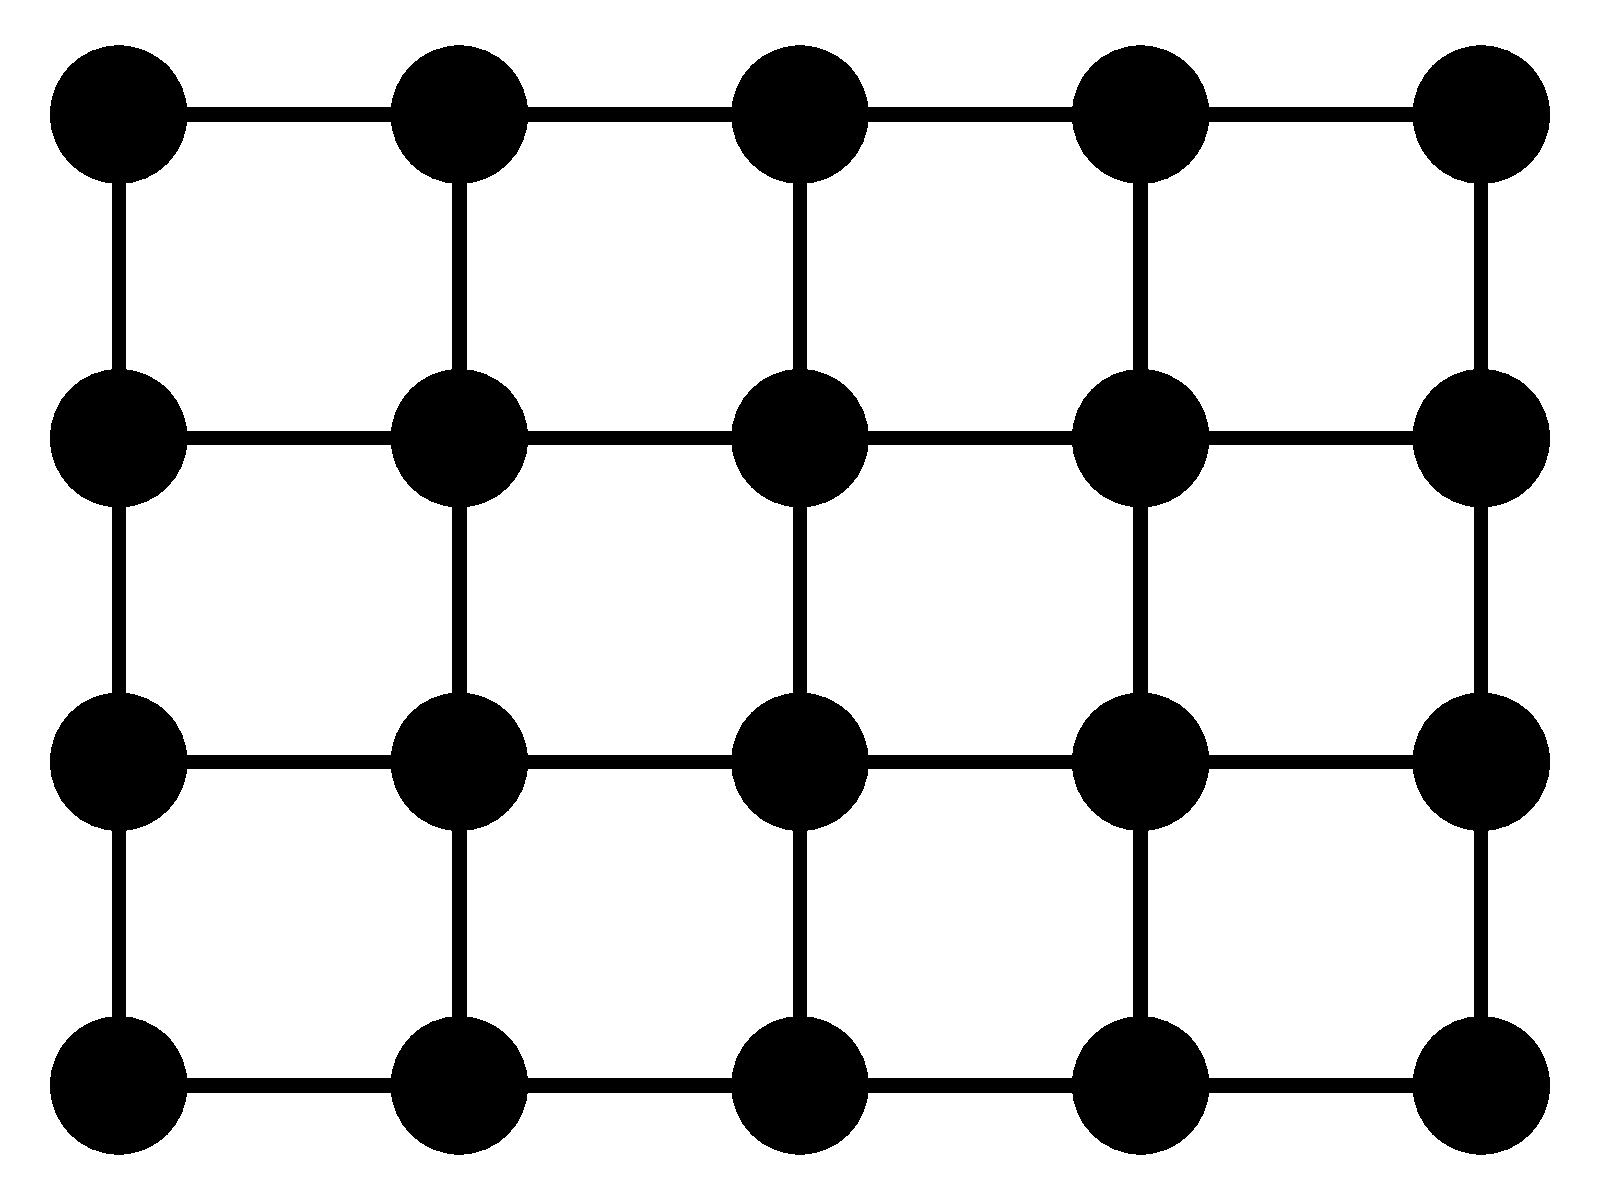
\includegraphics[width=\textwidth]{Images/uniform.pdf}
    \caption{uniform}
    \label{fig:uniform}
  \end{subfigure}
  \begin{subfigure}[b]{0.2\textwidth}
    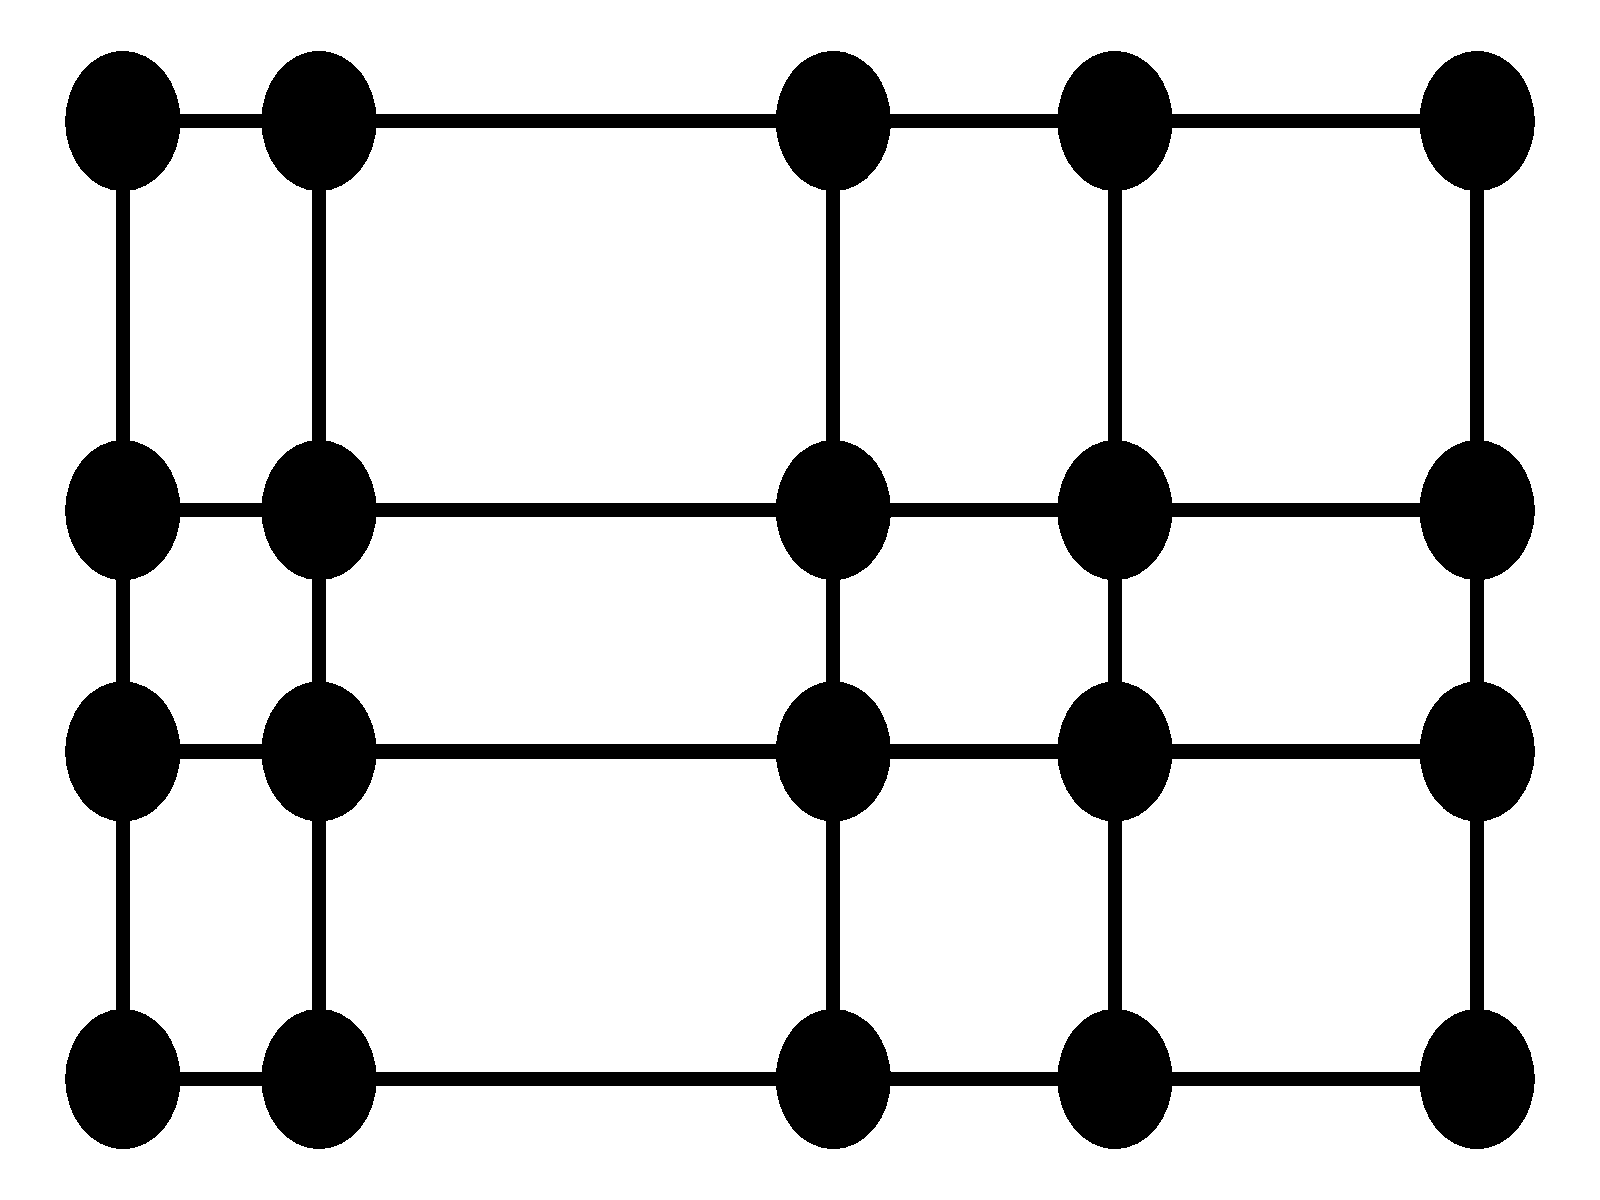
\includegraphics[width=\textwidth]{Images/rectilinear.pdf}
    \caption{rectilinear}
    \label{fig:rectilinear}
  \end{subfigure}
  \begin{subfigure}[b]{0.19\textwidth}
    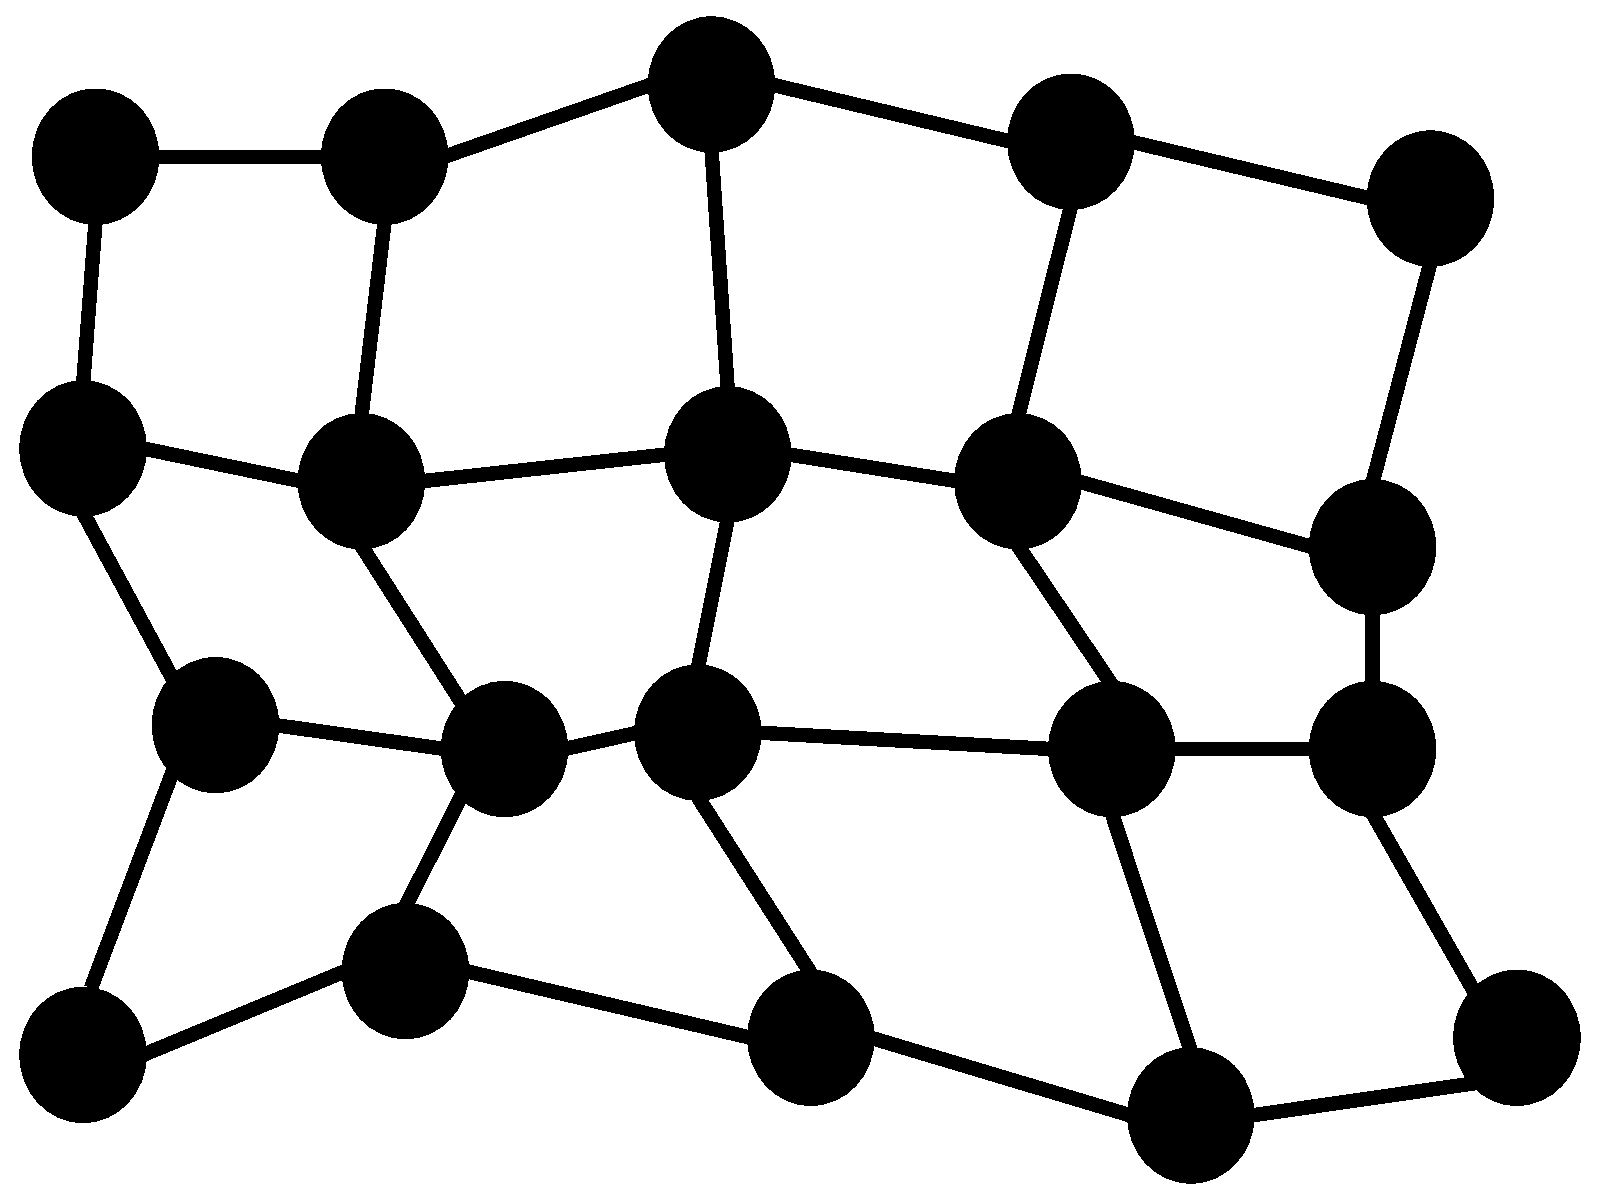
\includegraphics[width=\textwidth]{Images/curvilinear.pdf}
    \caption{curvilinear}
    \label{fig:curvilinear}
  \end{subfigure}
  \caption{Different types of grids. Uniform structured grids like in
  Figure~\ref{fig:uniform} can have varying distances inbetween
  dimensions, but along a dimension, the distances of the nodes are
  equal. Figure~\ref{fig:uniform}, \ref{fig:rectilinear} and
  \ref{fig:curvilinear} are variants of structured grids and therefore
  their connectivity is given by the ordering of the nodes.}
  \label{fig:grids}
\end{figure}

%%%%%%%%%%%%%%%%%%%%%%%%%%%%%%%%%%%%%%%%%%%%%%%%%%%%%%%%%%%%%%%%%%%%%%%%
\section{Scalar Fields}
%%%%%%%%%%%%%%%%%%%%%%%%%%%%%%%%%%%%%%%%%%%%%%%%%%%%%%%%%%%%%%%%%%%%%%%%

\begin{figure}
  \centering
  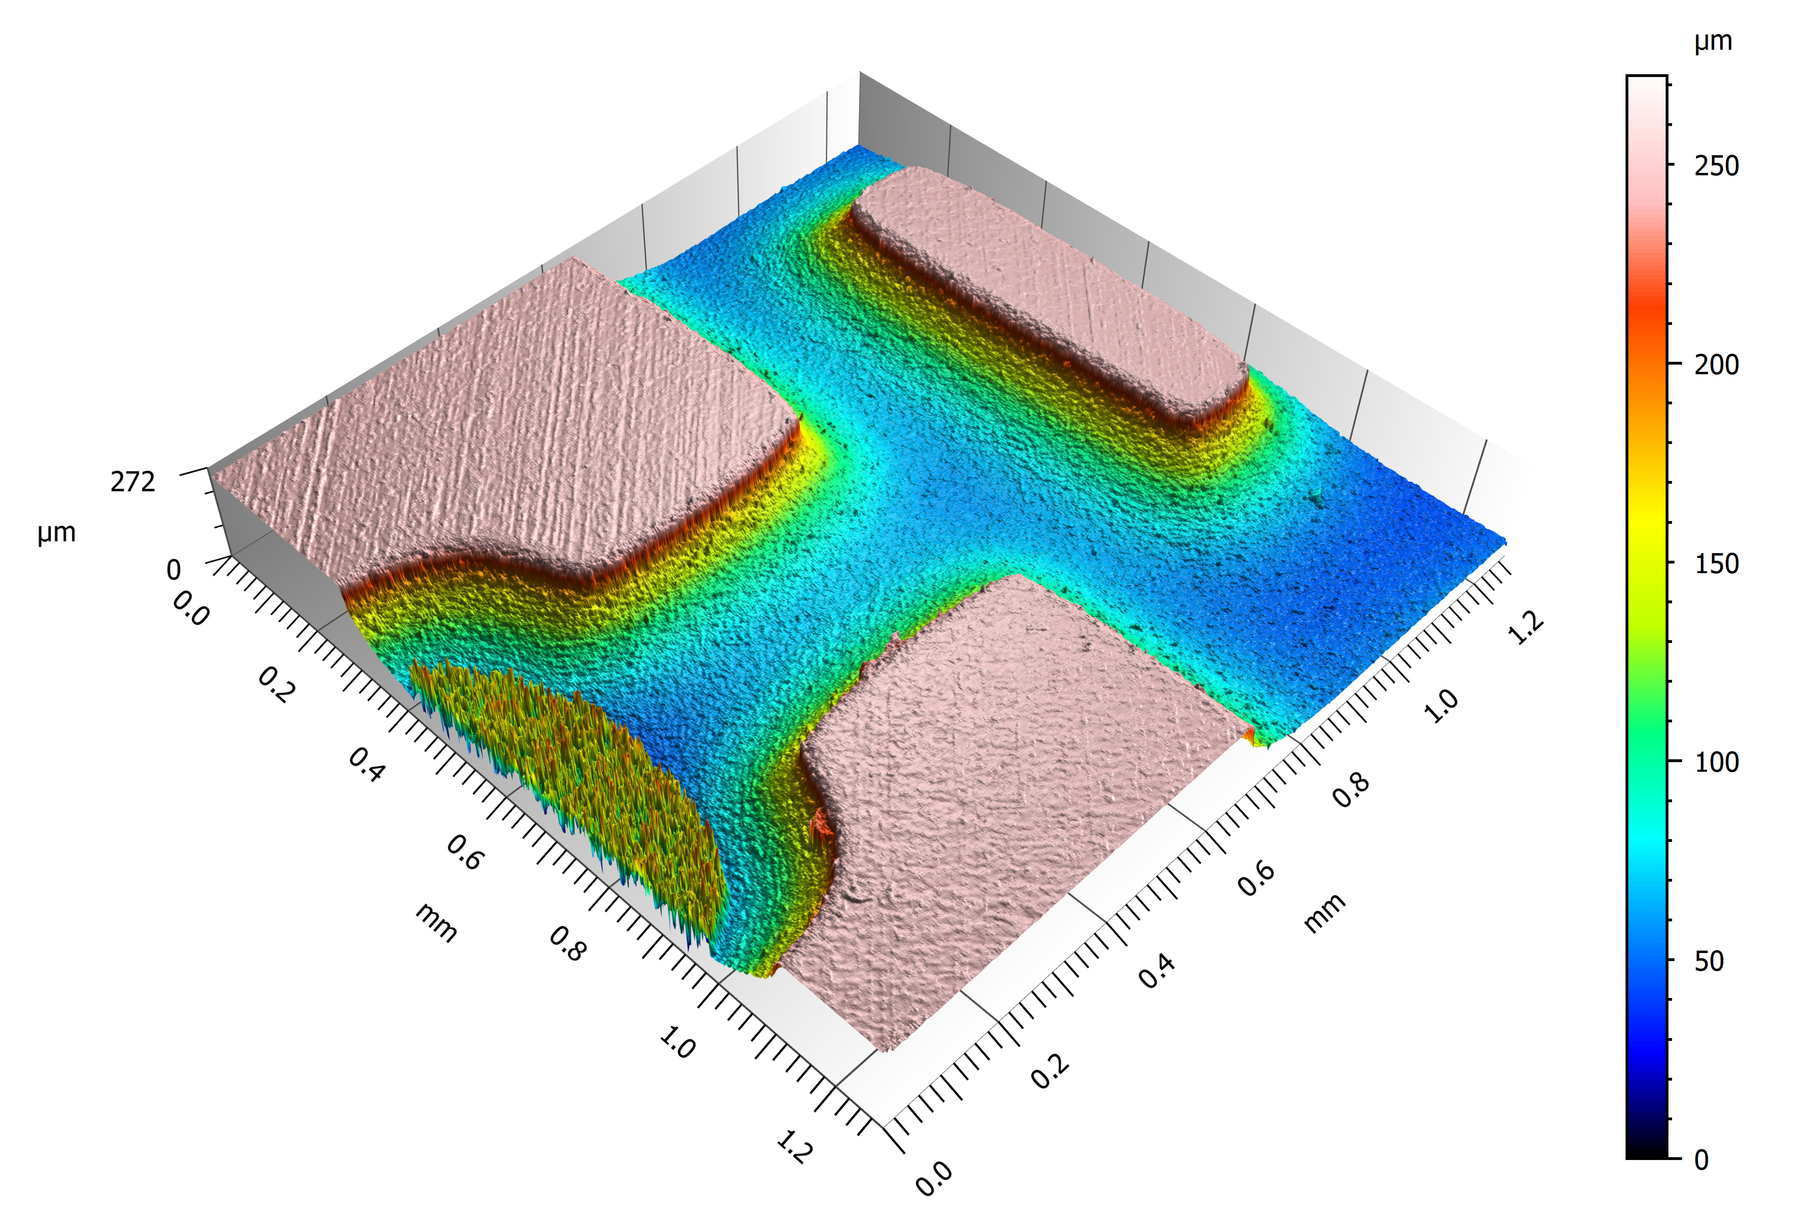
\includegraphics[width=0.85\textwidth]{Images/microfluid.png}
  \caption{3-dimensional view of a color coded 2-dimensional heightmap.
  The color scale to the right gives information on the height values in
  the visualization. This image shows a part of a microfluidic channel,
  observed with a microscope. Microfluidics deal with the manipulation
  and controlling of fluids in the range of micro- to pictoliters.
  Picture from ZEISS Microscopy~\cite{HM}.}
  \label{fig:HM}
\end{figure}

An $n$-dimensional field with a single scalar value at every point in
space is called a scalar field. A simple example for a scalar field is a
height map of some geographical terrain. It has two dimensions with a
height value at every point, usually encoded with color (Figure
\ref{fig:HM}). In this work we will use the notation $S(x)$ for the
scalar value at point $\text{x} = (x_1,\dots,x_n)$ in the scalar field $S$ with
$S: \real^n \rightarrow \real$. While in continuous scalar fields the
value of every point is defined by a function, discrete scalar fields
only have values at specific points in space. As real world data is
often acquired by measuring certain locations and usually does not
follow any graspable function, we will focus on uniformly structured
discrete scalar fields in this work, where $n \in \{2,3\}$. This also
applies to the other types of fields we will encounter, because they
have the same resolution as the scalar field.

%%%%%%%%%%%%%%%%%%%%%%%%%%%%%%%%%%%%%%%%%%%%%%%%%%%%%%%%%%%%%%%%%%%%%%%%
\section{Vector Fields}
%%%%%%%%%%%%%%%%%%%%%%%%%%%%%%%%%%%%%%%%%%%%%%%%%%%%%%%%%%%%%%%%%%%%%%%%

An $n$-dimensional vector field $V$ associates an $m$-dimensional vector
with every point in space $V(x_1,\dots,x_n):\real^n \rightarrow \real^m$.
If the vector field is the result of deriving a scalar field, thus the 
vector field is the gradient of the scalar field, the vector field is
called conservative. Conservative vector fields have the property, that
the line integral along any path connecting two points is always equal.
Since we are extracting features from scalar fields in this work, our
vector fields will always be conservative and $n = m$.

%%%%%%%%%%%%%%%%%%%%%%%%%%%%%%%%%%%%%%%%%%%%%%%%%%%%%%%%%%%%%%%%%%%%%%%%
\section{Tensor Fields}
%%%%%%%%%%%%%%%%%%%%%%%%%%%%%%%%%%%%%%%%%%%%%%%%%%%%%%%%%%%%%%%%%%%%%%%%

An $n$-dimensional tensor field $H$ associates an arbitrarily
dimensional tensor with every point in space $H(x_1,\dots,x_n): \real^n
\rightarrow \real^{m_1 \times \cdots \times m_k}$, where $k \in
\mathbb{N}$ is the rank of the tensor. Tensor fields are a
generalization of scalar and vector fields as a tensor of rank 0 would
represent a scalar and a tensor of rank 1 a vector. In our case, besides
scalars and vector, the tensors we encounter are of rank 2 and therefore
matrices in $\real^ {m \times l}$. As we will see later, the matrices
are covariance and Hessian matrices and therefore quadratic per
definition with $m = l$.

%%%%%%%%%%%%%%%%%%%%%%%%%%%%%%%%%%%%%%%%%%%%%%%%%%%%%%%%%%%%%%%%%%%%%%%%
\section{Linear Interpolation}
%%%%%%%%%%%%%%%%%%%%%%%%%%%%%%%%%%%%%%%%%%%%%%%%%%%%%%%%%%%%%%%%%%%%%%%%

\begin{figure}
  \centering
  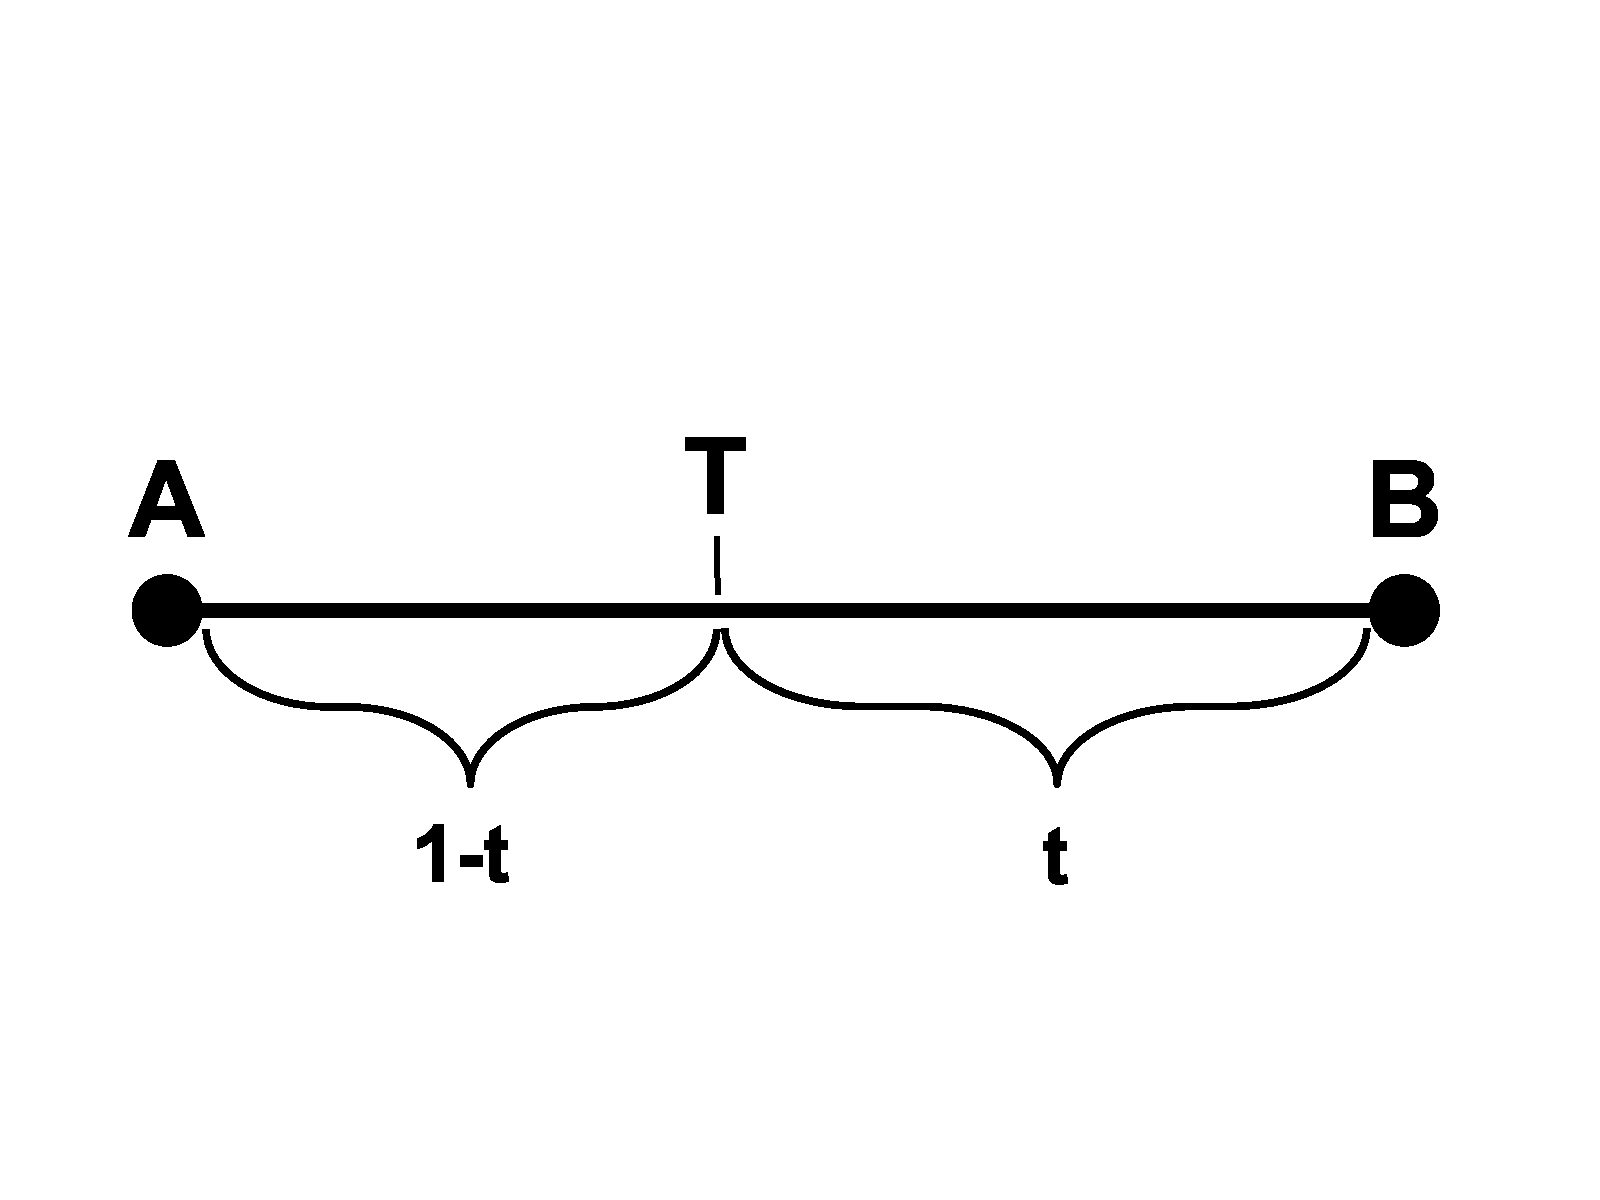
\includegraphics[width=0.5\textwidth]{Images/linipol.pdf}
  \caption{Tensors $A$ and $B$ at nodes in a discrete field. Linear
  interpolation can be thought of as a percentage mixing of two tensors.
  Therefore if the Tensor $T$ we want to interpolate is for
  example at $20\%$ of the distance between $A$ and $B$, we add $80\%$
  of $A$ to $20\%$ of $B$, as $T$ is more influenced by $A$,
  because of its proximity.}
  \label{fig:ipol}
\end{figure}

Our discrete fields only provide information for a limited number of
points along a dimension, therefore we need to estimate values lying
between known locations. To ease computation we assume that the
underlying functions of the fields are linear, allowing us to use simple
linear interpolation. As we will explain in Chapter~\ref{chap:Method},
we will only interpolate between neighboring nodes of a cell and can
therefore assume their distance to be 1. As we can express two
neighboring scalars, vectors or matrices as tensors of rank 2 with $A, B
\in \real^{n \times m}$ and $n,m \in \{1,2,3\}$, we generalize the
interpolation to:
\begin{equation}
  T =
  \begin{bmatrix}
    (1-t) \cdot A_{11} + t \cdot B_{11} & \dots & (1-t) \cdot A_{n1} + t \cdot B_{n1} \\
    \vdots & \ddots & \vdots \\
    (1-t) \cdot A_{1m} + t \cdot B_{1m} & \dots & (1-t) \cdot A_{nm} + t \cdot B_{nm} \\
  \end{bmatrix}
  \in \real^{n \times m},
\end{equation}
with $T$ being the interpolated tensor at the relative distance $t$ to
tensor $B$ (see Figure~\ref{fig:ipol}).

%%%%%%%%%%%%%%%%%%%%%%%%%%%%%%%%%%%%%%%%%%%%%%%%%%%%%%%%%%%%%%%%%%%%%%%%
\section{Derivatives}\label{sec:derivatives}
%%%%%%%%%%%%%%%%%%%%%%%%%%%%%%%%%%%%%%%%%%%%%%%%%%%%%%%%%%%%%%%%%%%%%%%%

Since we are dealing with discrete scalar fields, we have no function we
could derive to get the underlying gradient field. Instead we have to
approximate the derivatives with finite difference methods. There are
three forms which are commonly used:\\
\begin{inparaenum}[(a)]
  \item Forward Differences
  \begin{equation}
    \nabla f(x_i) = \frac{f(x_{i+1}) - f(x_i)}{h},
  \end{equation}
  \item Backward Differences
  \begin{equation}
    \nabla f(x_i) = \frac{f(x_i) - f(x_{i-1})}{h},
  \end{equation}
  \item Central Differences
  \begin{equation}\label{eq:centDiff}
    \nabla f(x_i) = \frac{f(x_{i+1}) - f(x_{i-1})}{2h},
  \end{equation}
\end{inparaenum}
where $f(x_i)$ denotes the $i$-th point of the function $f(x): \real
\rightarrow \real$ and $h$ the distance between two neighboring points.
Forward and backward differences are used at the borders of the field,
where no previous or succeeding point is available. As we will explain
in Chapter~\ref{chap:Method}, with our current implementation we process
cells with a fixed size and therefore do not consider border cases, thus
this work focuses on central differences.

%----------------------------------------------------------------------%
\subsection{First Derivative}
%----------------------------------------------------------------------%

When deriving an $n$-dimensional scalar field $S$, we need to apply
Equation~\ref{eq:centDiff} for every dimension. This results in $n$
scalar values, representing the change of the scalar field in the
respective dimension. These values can be interpreted as an
$n$-dimensional vector, the gradient, pointing in the direction of
greatest ascend for every point of the scalar field. This is the
vector field $\nabla S(x)$.

%----------------------------------------------------------------------%
\subsection{Second Derivative}
%----------------------------------------------------------------------%

The second derivative of an $n$-dimensional scalar field is an $n$
-dimensional tensor field with $\nabla^2 S:\real^n \rightarrow \real^{n
\times n}$. This tensor field can again be obtained with the central
difference method applied to every dimension of the gradient field. Here
we get an $n$-dimensional vector per dimension as we are subtracting the
previous gradient from the succeeding gradient of point $x$ along any
dimension. These vectors represent the respective columns of the so
called Hessian matrix. The Hessian matrix $H$ is a specification of the
Jacobian Matrix $J$, which derives any vector valued function $f(x):
\real^n \rightarrow \real^m$, $J \in \real^{m \times n}$. The Hessian
matrix is obtained when deriving a conservative vector field, therefore
the Hessian is quadratic with:

\begin{equation}
  H =
  \begin{bmatrix}
    \frac{\partial^2 S}{\partial x_1^2} & \frac{\partial^2 S}{\partial x_1 \partial x_2} & \dots & \frac{\partial^2 S}{\partial x_1 \partial x_n}\\
    \frac{\partial^2 S}{\partial x_2 \partial x_1} & \frac{\partial^2 S}{\partial x_2^2} & \dots & \frac{\partial^2 S}{\partial x_2 \partial x_n}\\
    \vdots & \vdots & \ddots & \vdots \\
    \frac{\partial^2 S}{\partial x_n \partial x_1} & \frac{\partial^2 S}{\partial x_n \partial x_2} & \dots & \frac{\partial^2 S}{\partial x_n^2}
  \end{bmatrix}
  \in \real^{n \times n}.
\end{equation}

\noindent According to Schwarz's theorem of the symmetry of second
derivatives ([is wikipedia enough reference?]), the Hessian is assumed
to be symmetric, therefore the eigenvectors are orthogonal and the
eigenvalues are real valued. The eigenvalues of the Hessian denote the
second directional derivative of the scalar field along the direction of
the corresponding eigenvector, and thus the change of the gradient in
the direction of the eigenvector. The eigenvectors are the axis along
which the gradient changes the most and the eigenvalues determine by how
much. Independent of the direction taken along the eigenvector, a
negative eigenvalue pushes the gradient against the direction taken,
whereas a positive eigenvalue scales the gradient along its direction.
Figure~\ref{fig:gradEV} explains this relation on a simple example.
\begin{figure}
  \centering
  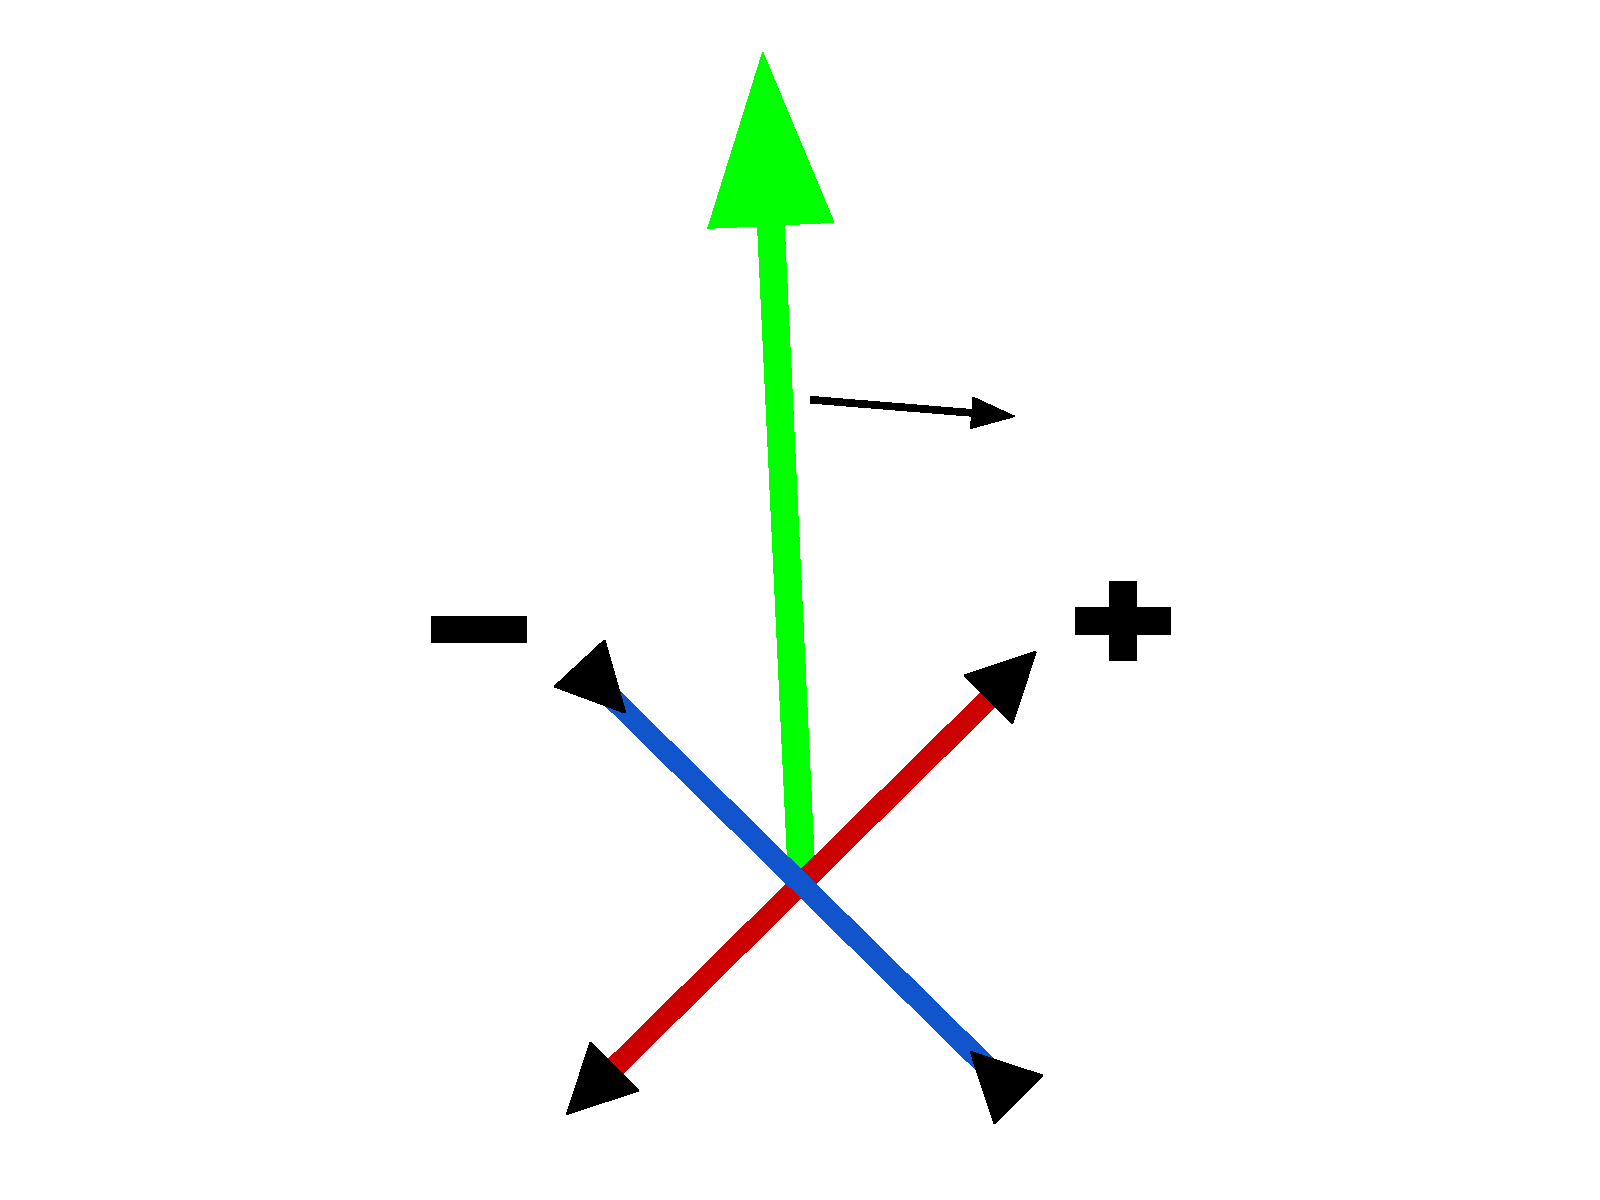
\includegraphics[width=0.7\textwidth]{Images/gradEV.pdf}
  \caption{Influence of the eigenvectors and the sign of their
  eigenvalues on the gradient (green) along their direction. The
  eigenvalues show us, that if we take a step along the direction of the
  gradient, the gradient turns into the direction depicted by the black
  arrow, as he is scaled along the red eigenvector and squished along
  the blue eigenvector.}
  \label{fig:gradEV}
\end{figure}

%%%%%%%%%%%%%%%%%%%%%%%%%%%%%%%%%%%%%%%%%%%%%%%%%%%%%%%%%%%%%%%%%%%%%%%%
\section{Uncertain Scalar Fields}\label{sec:USF}
%%%%%%%%%%%%%%%%%%%%%%%%%%%%%%%%%%%%%%%%%%%%%%%%%%%%%%%%%%%%%%%%%%%%%%%%

\begin{figure}
  \centering
  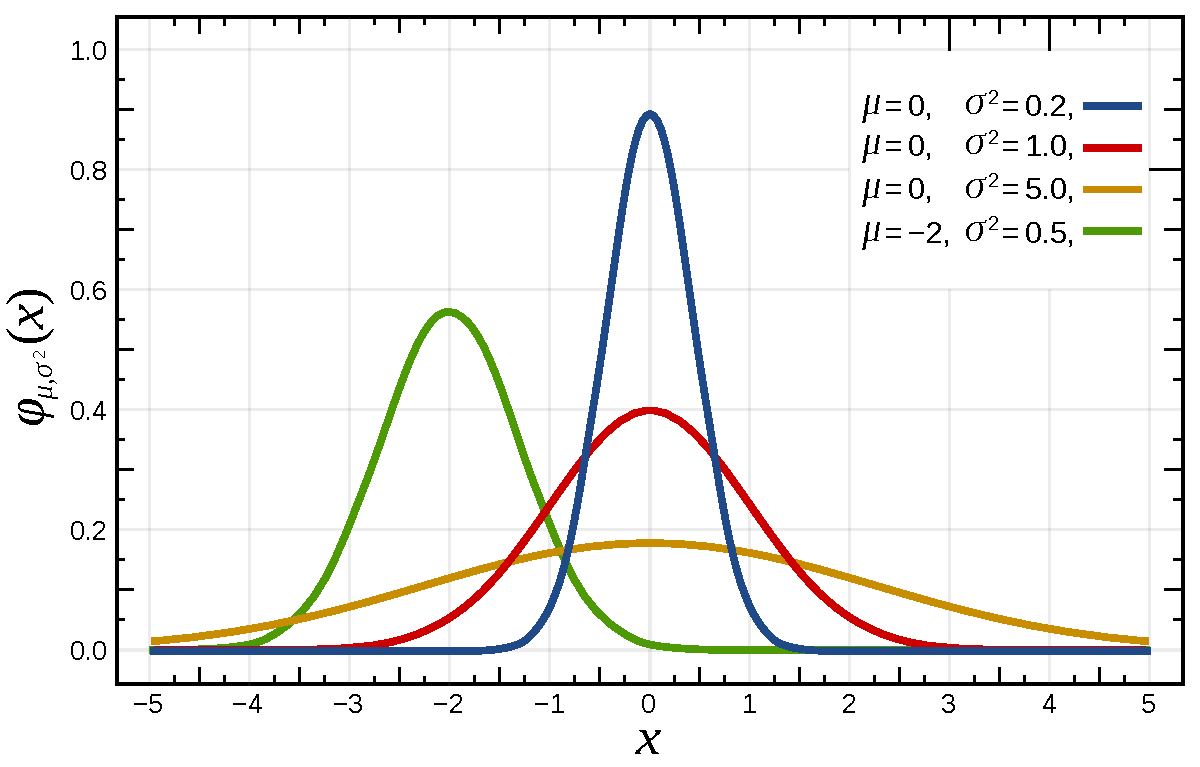
\includegraphics[width=0.75\textwidth]{Images/gauss.pdf}
  \caption{Probability density function for a random variable $X$ from a
   Gaussian distribution for different values of the mean and variance.
   Low variance (blue) equals a high probability for values close to the
   mean, whereas high variance (yellow) leads to wider spread
   probabilities. The mean value determines the peak of the probability
   curve. The red curve shows a standard normal distribution with mean
   $\mu = 0$ and variance $\sigma^2 = 1$. Image from Wikipedia
   \cite{Gauss}.}
   \label{fig:gauss}
\end{figure}

In computer science, simulations are more and more used to model real
world problems, making use of todays computational power. For example, a
common way to estimate the weather of the following days is to run
multiple simulations with slightly changing parameters. Such simulations
lead to sets of correlated fields with slight differences between the
members of the ensemble. Analyzing every member individually and
comparing them to the others is infeasible, which raises the need for a
simultaneous analysis of the results. As we are extracting features from
scalar fields, we introduce the uncertain scalar field, containing the
information about the distribution of the data. Many physical phenomena
are modeled with Gaussian (normal) distributions. A Gaussian
distribution assumes that the data is distributed around a mean $\mu$
with standard deviation $\sigma$ and variance $\sigma^2$. The
probability for the value of a variable $X$ from the distribution is
given by the probability density function

\begin{equation}
  \phi_{\mu, \sigma^2}(X) = \frac{1}{\sqrt{2 \pi \sigma^2}} e^{-\frac{(X - \mu)^2}{2 \sigma^2}},
\end{equation}

assigning a higher probability to values closer to the mean, leading to
the characteristic Gauss bells visible in Figure~\ref{fig:gauss}. To
obtain our uncertain scalar field, we give it the same resolution as the
members of the ensemble, assuming they have equal resolutions, and
calculate the mean and the variance for every point of the field. The
mean is defined as $\mu_x = \frac{1}{m} \sum_{k=1}^m S_k(x)$ and the
variance as $\sigma_x^2 = \frac{1}{m} \sum_{k=1}^m (S_k(x)-\mu_x)^2$ and
therefore our uncertain scalar field as

\begin{equation}
  S_{\mathcal{N}}(x) = \mathcal{N}(\mu_{x}, \sigma_{x}^2),
\end{equation}

\noindent for the $m$ entities at point $x = (x_1,\dots,x_n)$.

(tobechanged)
As they also pointed out in their work, we need to consider the
neighborhood of $x$, so that the derivatives of the uncertain scalar
field are Gaussian distributed as well. As we will explain in
Chapter~\ref{chap:Method}, we will search for ridges
(Section~\ref{sec:Ridges}) inside cells. Therefore, combining this with
the need for neighboring points, we have 4 (or 8 in the 3D case) nodes
of the cell we want to observe, together with their neighboring points
in every dimension and, because we also want to calculate the second
derivative, their neighboring nodes as well. Cleared from redundant
points, this results in 24 (80) nodes per neighborhood as illustrated in
Figure~\ref{fig:NH}. We can take this neighborhood as a vector $v_x$ and
calculate the $24$-dimensional mean vector at point $x$ of the mean
vector field $\mu(x) = \frac{1}{m} \sum_{k=1}^m v_{x,k}$, followed by
the $24 \times 24$-dimensional covariance matrix, with the covariance
field being $\Sigma(x)= \frac{1}{m} \sum_{k=1}^m (v_{x,k} -
\mu(x)){(v_{x,k} - \mu{(x)})}^\top$. Therefore our uncertain scalar
fields follows a multivariate Gaussian distribution at every location

\begin{equation}
  S_{\mathcal{N}}(x) = \mathcal{N}(\mu(x), \Sigma(x)).\\
\end{equation}

\begin{figure}
  \centering
  \begin{subfigure}[b]{0.4\textwidth}
    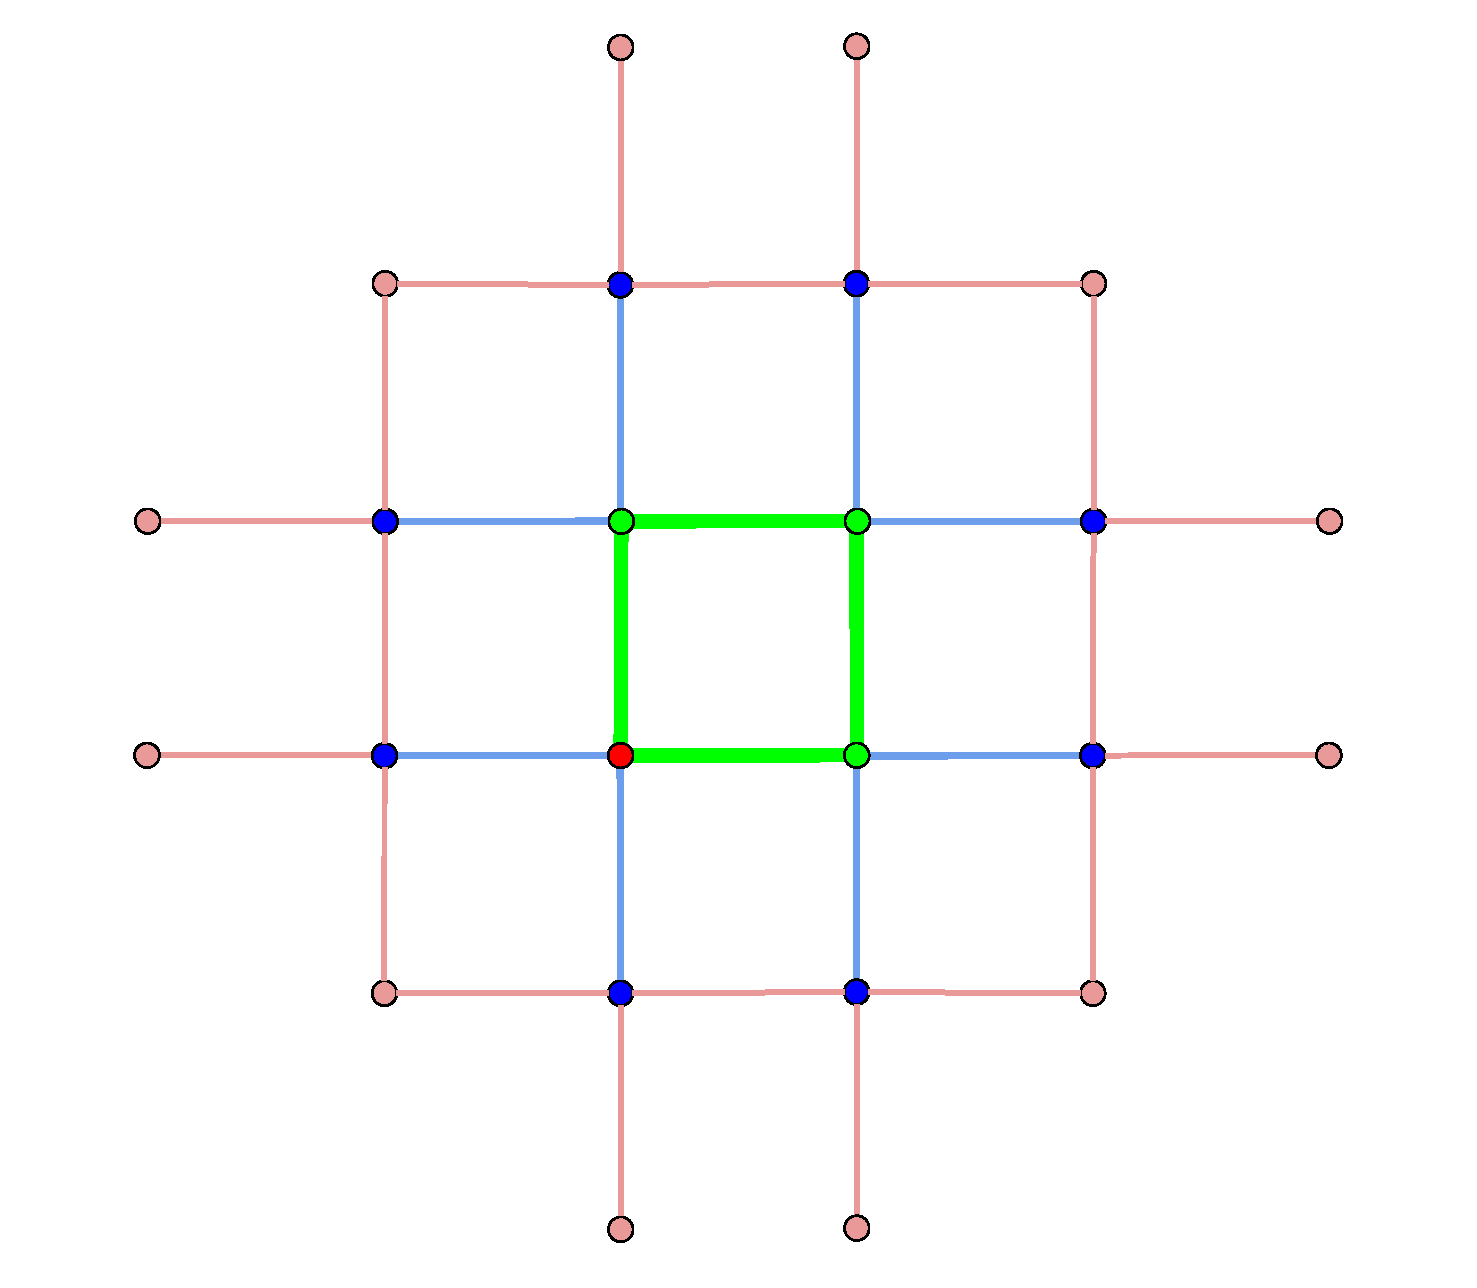
\includegraphics[width=\textwidth]{Images/2DNH.pdf}
    \caption{2D neighborhood}
    \label{fig:2DNH}
  \end{subfigure}
  \begin{subfigure}[b]{0.49\textwidth}
    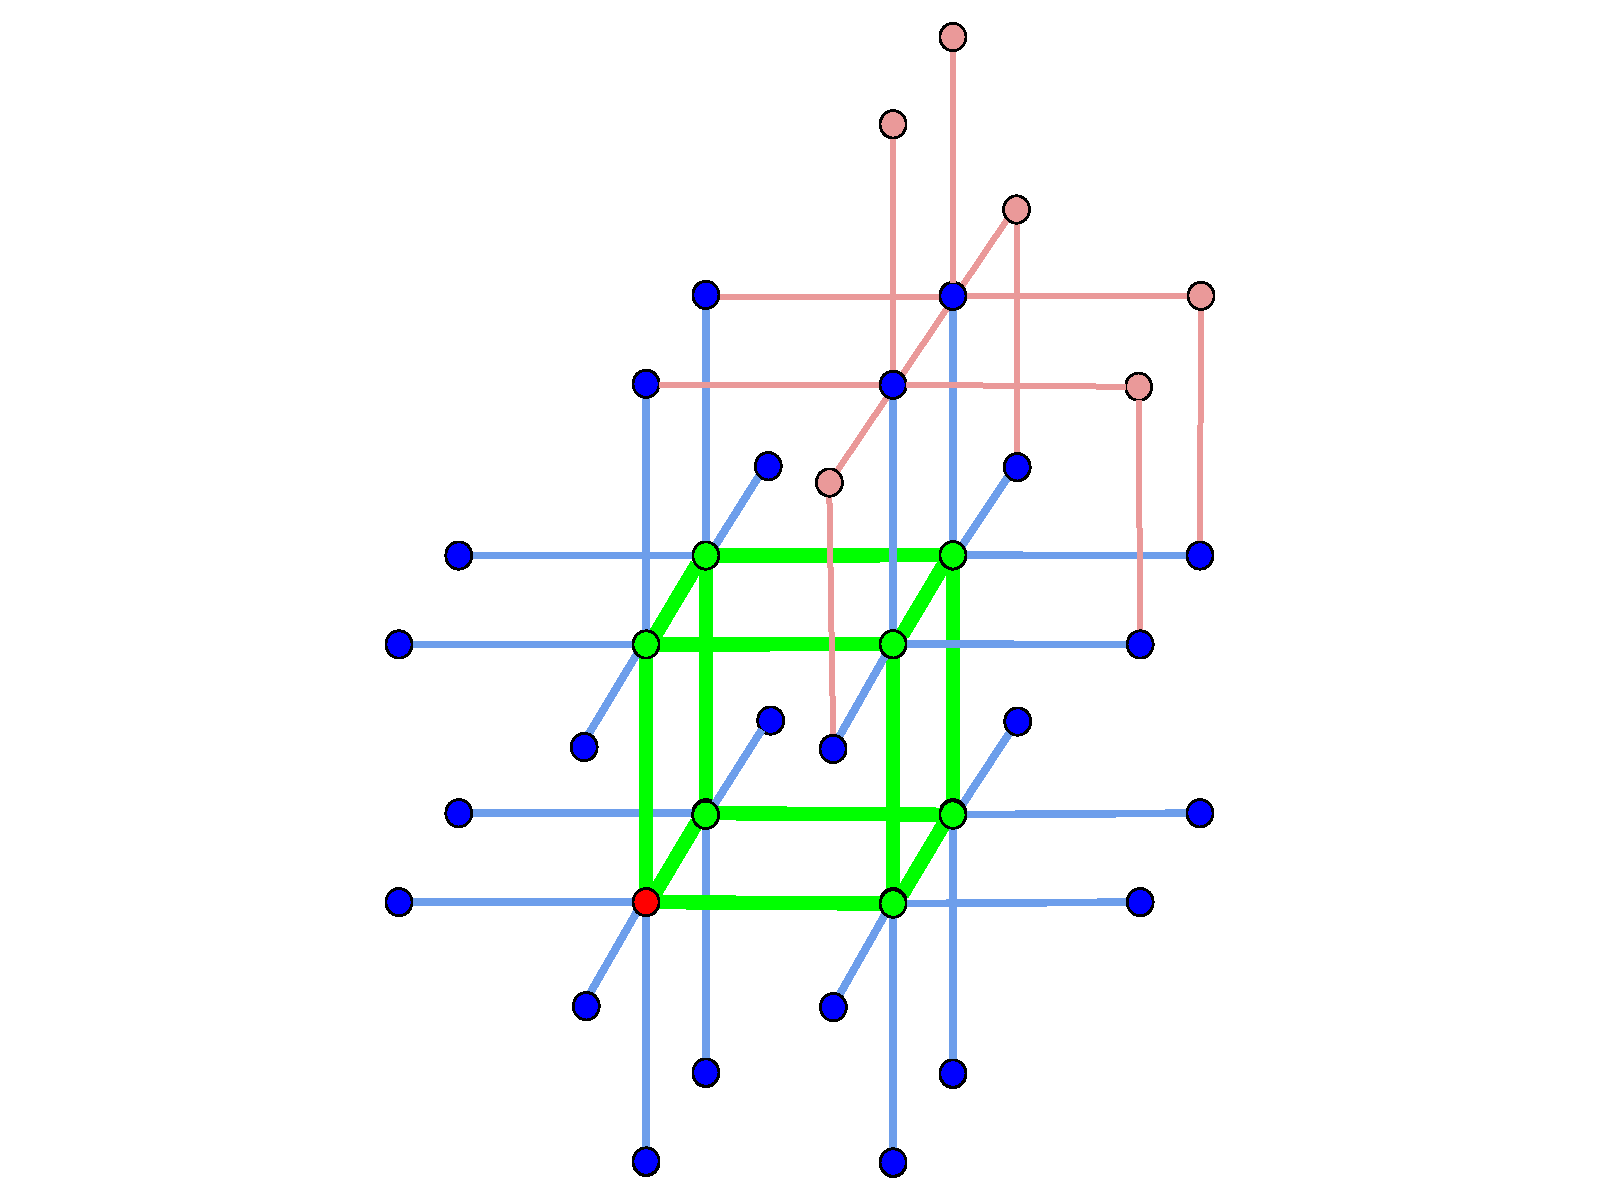
\includegraphics[width=\textwidth]{Images/3DNH.pdf}
    \caption{3D neighborhood}
    \label{fig:3DNH}
  \end{subfigure}
  \caption{Support regions for the 2- and 3-dimensional case. A cell of
  this size is created for every node of the initial scalar fields,
  depending on the dimensionality of the data set. The red node marks
  the location of the actual node at this position in the scalar field,
  the green nodes belong to the cell we want to inspect and the blue
  nodes are used to calculate the gradient of the green nodes via
  central differences, as well as the gradient of the red node of
  course. The outer pink nodes are used for the gradient of the blue
  ones and with their gradient we can estimate the Hessian
  matrices of the cell nodes. The neighboring points of the blue nodes
  in Figure~\ref{fig:3DNH} are only drawn for the two upper right ones,
  as drawing all of them would make the image too cluttered.}
  \label{fig:NH}
\end{figure}

%%%%%%%%%%%%%%%%%%%%%%%%%%%%%%%%%%%%%%%%%%%%%%%%%%%%%%%%%%%%%%%%%%%%%%%%
\section{Matrix Decompositions}
%%%%%%%%%%%%%%%%%%%%%%%%%%%%%%%%%%%%%%%%%%%%%%%%%%%%%%%%%%%%%%%%%%%%%%%%

A matrix decomposition is a factorization of a matrix into its
constituent parts. In general there are two classes of factorizations:
decompositions used for solving linear equations and decompositions
based on eigenvalues and vectors. We will consider one example from each
class, namely the Cholesky and the Eigendecomposition. As we will
explain in Section~\ref{sec:MGS} we will use both decompositions to
generate samples from a multivariate gaussian distribution, even though
they are from different classes.

%----------------------------------------------------------------------%
\subsection{Cholesky Decomposition}\label{sec:cholesky}
%----------------------------------------------------------------------%

The Cholesky factorization is a decomposition of a square, hermititan,
positive definite matrix $A$ into the product of a lower-triangular
matrix L and its conjugate transpose $A = L L^*$. A matrix $C$ is
hermitian if the diagonal elements are real valued and $C_{ij} =
\overline{C}_{ji}$, meaning that $\overline{C}_{ji}$ is the complex
conjugate of $C_{ij}$. Two complex numbers are complex conjugate if they
have equal real and imaginary parts, but opposite signs. For example,
$1+i \in \mathbb{C}$ is the complex conjugate of $1-i$. Following this
property, the standard Cholesky decomposition is also applicable for
every real valued, symmetric, positive definite matrix, resulting in a
lower triangular real valued matrix and its transpose $A = L L^\top$. We
will only deal with real valued matrices in this work and therefore
follow this notation. A simple way to determine the definiteness of a
matrix is to look at its eigenvalues. If every eigenvalue $\lambda$ of a
square $n \times n$ matrix is greater than zero, $\lambda_{i} > 0, i \in
\{1,\dots,n\}$, the matrix is positive definite. If every eigenvalue is
greater or equal to zero, $\lambda_{i} \ge 0$, the matrix is positive
semi-definite. The same goes for negative eigenvalues, as they make the
matrix negative (semi-) definite.

%----------------------------------------------------------------------%
\subsubsection{$LDL^T$ Decomposition}
%----------------------------------------------------------------------%

The closely related $LDL^T$ decomposition extends the classical Cholesky
decomposition to semi-definite and negative definite matrices $A = L D
L^\top$, where $L$ is a lower unitriangular matrix, meaning there are
only ones on the diagonal, and $D$ is a diagonal matrix. The two
decompositions are related as follows:

\begin{equation}\label{eq:LDL}
  A = LDL^\top = (L D^\frac{1}{2}) (D^\frac{1}{2}  L^\top).
\end{equation}

\noindent This version has the advantage that it avoids extracting
square roots, thus allowing for negative entries in $D$, as it is
possible for some indefinite matrices for which no classical
decomposition exists, while having the same computational complexity as
the Cholesky decomposition. If the solution of a linear system is needed
and the system can be put into a symmetric form, the Cholesky
decomposition and its variant is the method of choice, as it offers
efficiency and usually numerical stability. Here is an example for both
variants of the decomposition:\\
\begin{inparaenum}[]
  \item Cholesky decomposition of a symmetric real valued matrix
  \begin{equation}
    \begin{pmatrix}
      9 & 18 & -27\\
      18 & 40 & -18 \\
      -27 & -18 & 406
    \end{pmatrix}
    =
    \begin{pmatrix}
      3 & 0 & 0\\
      6 & 2 & 0 \\
      -9 & 18 & 1
    \end{pmatrix}
    \begin{pmatrix}
      3 & 6 & -9\\
      0 & 2 & 18 \\
      0 & 0 & 1
    \end{pmatrix}
  \end{equation}
  \item $LDL^T$ decomposition of the same matrix
  \begin{equation}
    \begin{pmatrix}
      9 & 18 & -27\\
      18 & 40 & -18 \\
      -27 & -18 & 406
    \end{pmatrix}
    =
    \begin{pmatrix}
      1 & 0 & 0\\
      2 & 1 & 0 \\
      -3 & 9 & 1
    \end{pmatrix}
    \begin{pmatrix}
      9 & 0 & 0\\
      0 & 4 & 0 \\
      0 & 0 & 1
    \end{pmatrix}
    \begin{pmatrix}
      1 & 2 & -3\\
      0 & 1 & 9 \\
      0 & 0 & 1
    \end{pmatrix}
    .
  \end{equation}
\end{inparaenum}

%----------------------------------------------------------------------%
\subsection{Eigendecomposition}\label{sec:eigen}
%----------------------------------------------------------------------%

The Eigendecomposition is a factorization of a square $n \times n$,
diagonizable matrix $A$, into the form $A = E \Lambda E^{-1}$, where the
columns of $E$ are $n$ linearly independent eigenvectors of $A$ and
$\Lambda$ is a diagonal matrix with the respective eigenvalues. The
eigenvalue $\lambda_i$ at $\Lambda_{ii}$ corresponds to the eigenvector
$\epsilon_i$ at column $i, i \in \{1,\dots,n\}$ of $E$. This follows the
basic attribute of eigenvectors, as they only change by a scalar factor
when multiplied with their respective matrix, meaning $A \epsilon =
\lambda \epsilon$ and therefore $A E = E \Lambda$, which leads to the
decomposition $A = E \Lambda E^{-1}$. Here is a simple example of the
Eigendecomposition of a symmetric, real, diagonizable matrix:

\begin{equation}
  \begin{pmatrix}
    1 & {-3} & 3\\
    3 & {-5} & 3\\
    6 & {-6} & 4
  \end{pmatrix}
  =
  \begin{pmatrix}
    1 & {-1} & 1\\
    1 & 0 & 1\\
    2 & 1 & 0
  \end{pmatrix}
  \begin{pmatrix}
    4 & 0 & 0\\
    0 & {-2} & 0\\
    0 & 0 & {-2}
  \end{pmatrix}
  \begin{pmatrix}
    0.5 & {-0.5} & 0.5\\
    {-1} & 1 & 0\\
    {-0.5} & 1.5 & {-0.5}
  \end{pmatrix}
  .
\end{equation}

\noindent An $n \times n$-dimensional matrix is diagonizable if it has
$n$ linearly independent eigenvectors. The decomposition can for example
be used to easily raise a matrix to a power, as you only have to raise
the eigenvalue matrix $\Lambda$ to that power:

\begin{equation}
  \begin{pmatrix}
    1 & {-3} & 3\\
    3 & {-5} & 3\\
    6 & {-6} & 4
  \end{pmatrix}
  ^4
  =
  E
  \Lambda^4
  E^{-1}
  =
  \begin{pmatrix}
    136 & {-120} & 120\\
    120 & {-104} & 120\\
    240 & {-240} & 256
  \end{pmatrix}
  .
\end{equation}

\noindent In this work, our matrices don't need to be diagonizable, as
this property is only required for the inverse of the eigenvector
matrix. Section~\ref{sec:MGS} will give more information on that matter.


%----------------------------------------------------------------------%
\subsubsection{Principal Component Analysis}
%----------------------------------------------------------------------%

\begin{figure}[t]
  \centering
  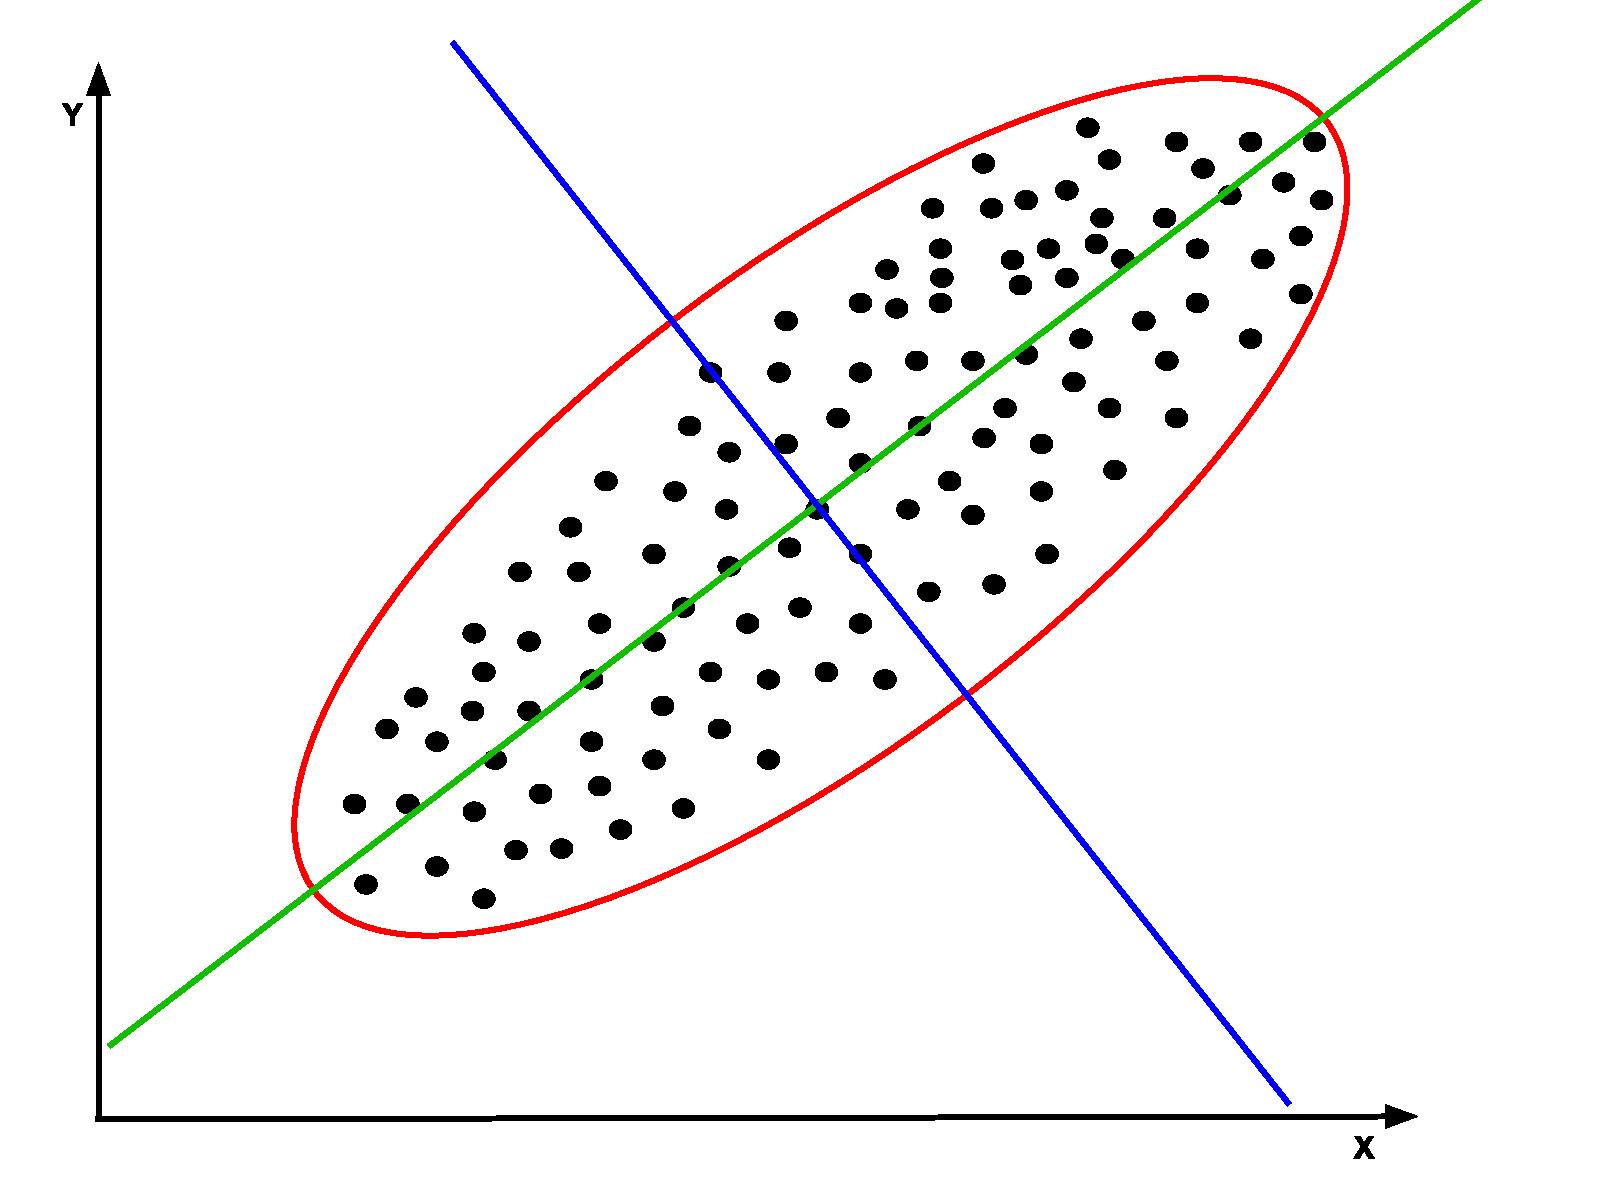
\includegraphics[width=0.75\textwidth]{Images/PCA.pdf}
  \caption{Principal Component Analysis of a set of points in
  $2$-dimensional space. The green line denotes the line of greatest
  variance, whereas the blue line is orthogonal to the green one and
  goes along the least variance. These lines correspond to the
  eigenvectors of a matrix containing the $x$ and $y$ coordinates of the
  points as columns.}
  \label{fig:PCA}
\end{figure}

Even though the Principal Component Analysis (PCA) is not a decomposition
in itself, it is an application of the Eigendecomposition. In general,
the PCA fits an $n$-dimensional ellipsoid around a set of possibly
correlated points. The first principle component then corresponds to the
axis of biggest magnitude of the ellipsoid and therefore the axis of the
largest variance of the data. The principal components are always
orthogonal to each other. When the Eigendecomposition is applied to
a matrix containing correlated points, the resulting eigenvectors match
the principal components, and the eigenvalues the variance along those
axes. See Figure~\ref{fig:PCA} for a graphical example.

%%%%%%%%%%%%%%%%%%%%%%%%%%%%%%%%%%%%%%%%%%%%%%%%%%%%%%%%%%%%%%%%%%%%%%%%
\section{Box-Muller Transformation}\label{sec:BM}
%%%%%%%%%%%%%%%%%%%%%%%%%%%%%%%%%%%%%%%%%%%%%%%%%%%%%%%%%%%%%%%%%%%%%%%%

The Box-Muller Transformation is a method to transform two uniformly
distributed random numbers into two independent, standard, normally
distributed random numbers. Let $U_1$ and $U_2$ be samples from the
uniform distribution on the interval ($0$, $1$). Let $N_1$ and $N_2$ be:

\begin{align}
  &N_1 = \sqrt{-2 \ln{U_1}} \cos (2 \pi U_2) \\
  &N_2 = \sqrt{-2 \ln{U_1}} \sin (2 \pi U_2).
\end{align}

\noindent Then $N_1$ and $N_2$ are independent random numbers with a
standard normal distribution, meaning that their mean is $\mu = 0$ and
standard deviation $\sigma = 1$. This transformation can be repeated to
generate standard normal distributed vectors of arbitrary length.

%%%%%%%%%%%%%%%%%%%%%%%%%%%%%%%%%%%%%%%%%%%%%%%%%%%%%%%%%%%%%%%%%%%%%%%%
\section{Ridges}\label{sec:Ridges}
%%%%%%%%%%%%%%%%%%%%%%%%%%%%%%%%%%%%%%%%%%%%%%%%%%%%%%%%%%%%%%%%%%%%%%%%

While the intuitive definition of a ridge would be a path along the
crest of a mountain with terrain falling off on either side, we focus on
a mathematical definition of ridges. In principal, a ridge is a local
maximum of an $n$-dimensional function. The maximum of the
$1$-dimensional function $f(x) = -x^2$ would be the $0$-dimensional
point at $x=0$, the ridge point (Figure~\ref{fig:ridge1D}). When we add
a dimension, the domain becomes a $2$-dimensional surface, and the ridge
point expands into a $1$-dimensional ridge line
(Figure~\ref{fig:ridge2D}). Adding another dimension turns the function
domain into a $3$-dimensional volume and the ridge into a
$2$-dimensional surface (Figure~\ref{fig:ridge3D}). In general, the
ridge is an $n-k$-dimensional manifold in an $n$-dimensional space for
$k=\{1, \dots, n\}$. This means that ridge points and lines also exist
in $3$-dimensional domains for example. This work focuses on ridges in
$2$ and $3$-dimensional domains.\\
To calculate the maximum, we need to derive the function and search for
the points where the derived function is $0$. The derived function
$f'(x)=-2x$ has only one zero at $x=0$. Now we only know that we have
found an extremum and need to check whether its a maximum or minimum by
looking at the second derivative $f''(x)=-2$. As $-2 < 0$, we now know
that the extremum is a maximum. The same principal is applicable for
ridges in higher dimensions. Here the first derivative at point $x$, the
gradient, lies in the subspace spanned by $n-k$ eigenvectors of the
Hessian, the second derivative, if $x$ is on an $n-k$ dimensional ridge.
In other words, the dot product of the gradient with the remaining $k$
eigenvectors is $0$, as the dot product is the scalar projection of two
vectors or a measurement for how much the gradient points into the
direction of the eigenvector. Keep in mind that the gradient always
points into the direction of greatest ascend. These eigenvectors
therefore have to be orthogonal to the gradient and the corresponding
eigenvalues have to be negative just like in the example above, as $x$
is a maximum along the directions of the $k$ eigenvectors, thus falls
off in their directions and only increases along the direction of the
$n-k$ eigenvectors. Figure~(INSERT REF) explains this connection on a
simple two dimensional example. The question remaining is how to decide
which eigenvectors denote the ridge domain. Eberly~\cite{Eberly} and
Lindeberg~\cite{Lindeberg} proposed two ways on how to sort the
eigenvalues $\lambda_i$ in order to pick the right corresponding
eigenvectors $\epsilon_i$:\\
\begin{inparaenum}[]
  \item Eberly
  \begin{equation}\label{eq:Eberly}
   \lambda_1 \leq \cdots \leq \lambda_n
  \end{equation}
  \item Lindeberg
  \begin{equation}
    \lvert \lambda_1 \rvert \geq \cdots \geq \lvert \lambda_n \rvert.
  \end{equation}
\end{inparaenum}
\noindent Lindebergs method extracts a subset of the ridge features
found by Eberly. Lindeberg discards a feature if there is along any
eigenvector an upward bend, denoted by a positive eigenvalue, that is
stronger than the downward bend along the $n-k$ eigenvectors found by
Eberly. For the definition of Eberly, an upward bend along the ridge is
irrelevant for its existence. This work will use Eberlys method and
therefore the principle definition for the existence of an $n-k$
dimensional ridge at point $x \in \real^n$ is:\\

\begin{equation}\label{eq:ridgeDot}
  \nabla S(x) \cdot \epsilon_1 = \cdots = \nabla S(x) \cdot \epsilon_{k} = 0
\end{equation}
\begin{equation}\label{eq:ridgeEV}
  \lambda_k < 0
\end{equation}

\noindent The counterpart to ridges are valleys. These can be obtained
by extracting ridges from the scalar field $-S(x)$ or by checking
Equation~\ref{eq:ridgeDot} for the eigenvectors corresponding to the
$k$ largest eigenvalues and $\lambda_k > 0$.
\begin{figure}
  \begin{subfigure}[b]{0.33\textwidth}
    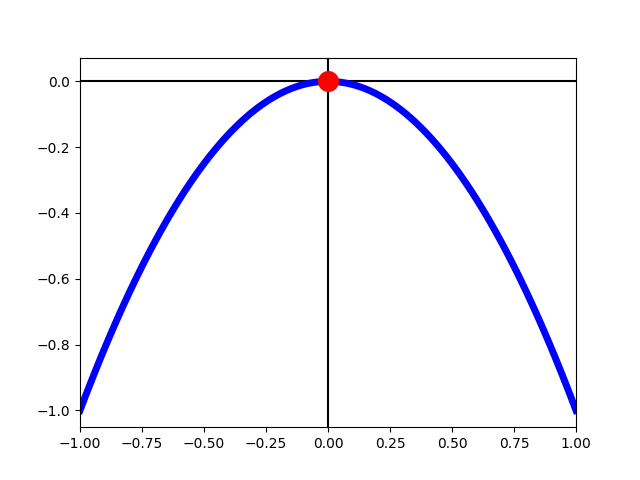
\includegraphics[width=\textwidth]{Images/func1D.png}
    \caption{$f(x)= -x^2$}
    \label{fig:ridge1D}
  \end{subfigure}
  \begin{subfigure}[b]{0.33\textwidth}
    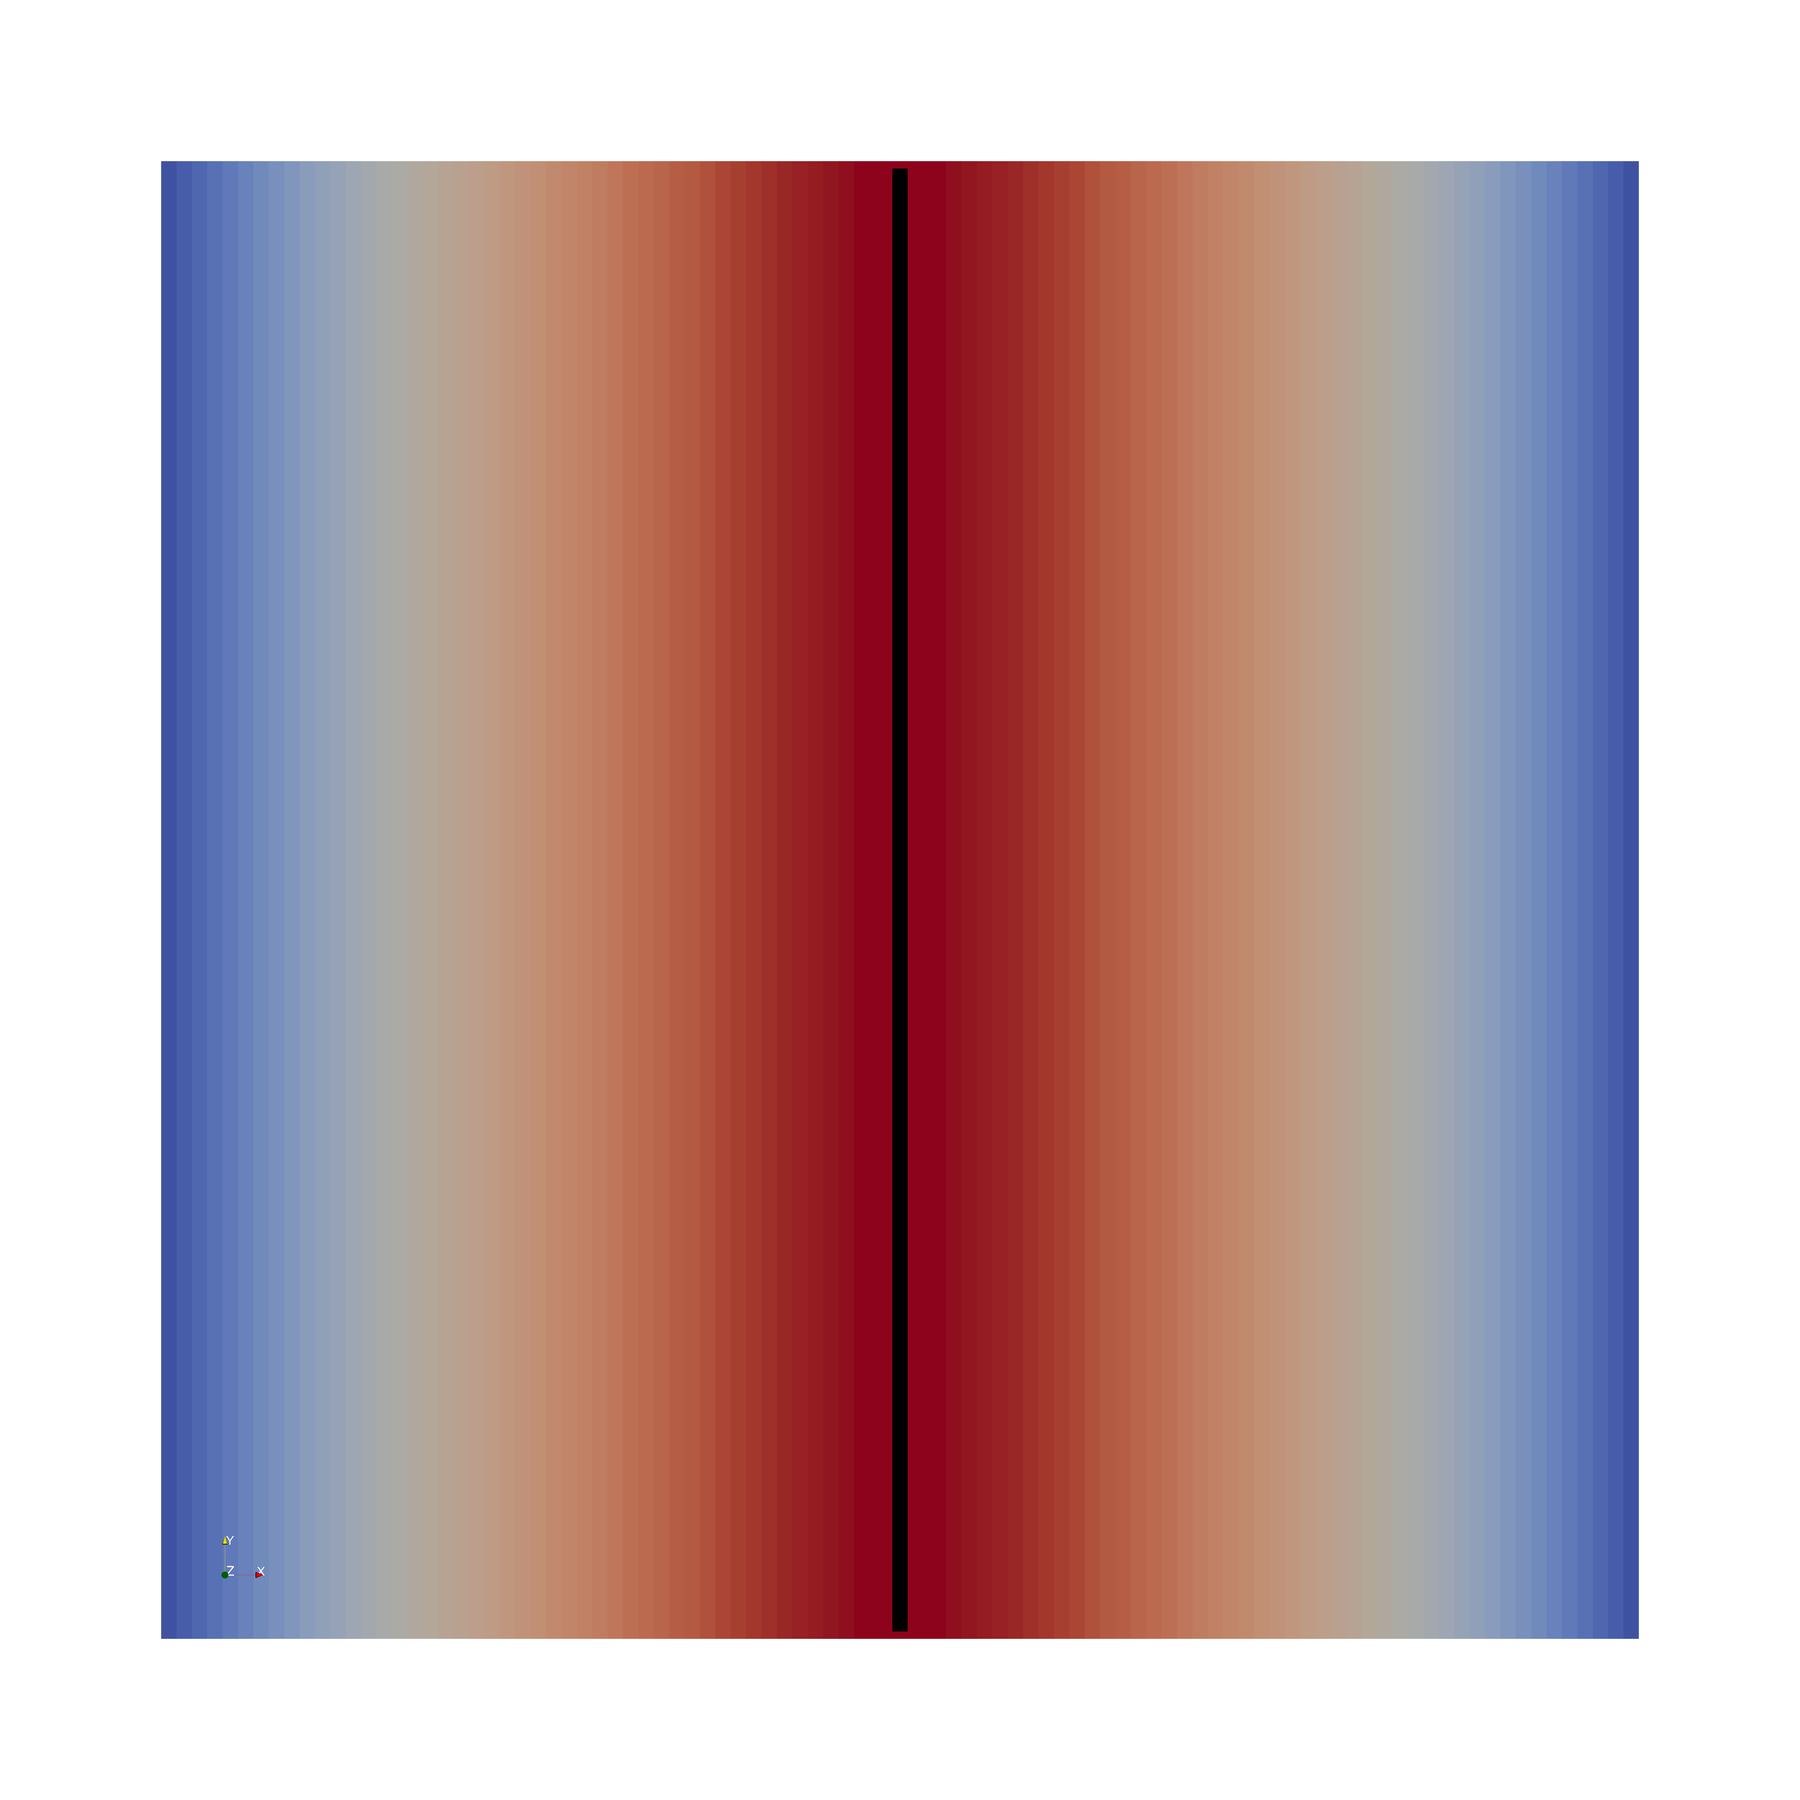
\includegraphics[width=\textwidth]{Images/func2D.png}
    \caption{$f(x,y)= -x^2$}
    \label{fig:ridge2D}
  \end{subfigure}
  \begin{subfigure}[b]{0.33\textwidth}
    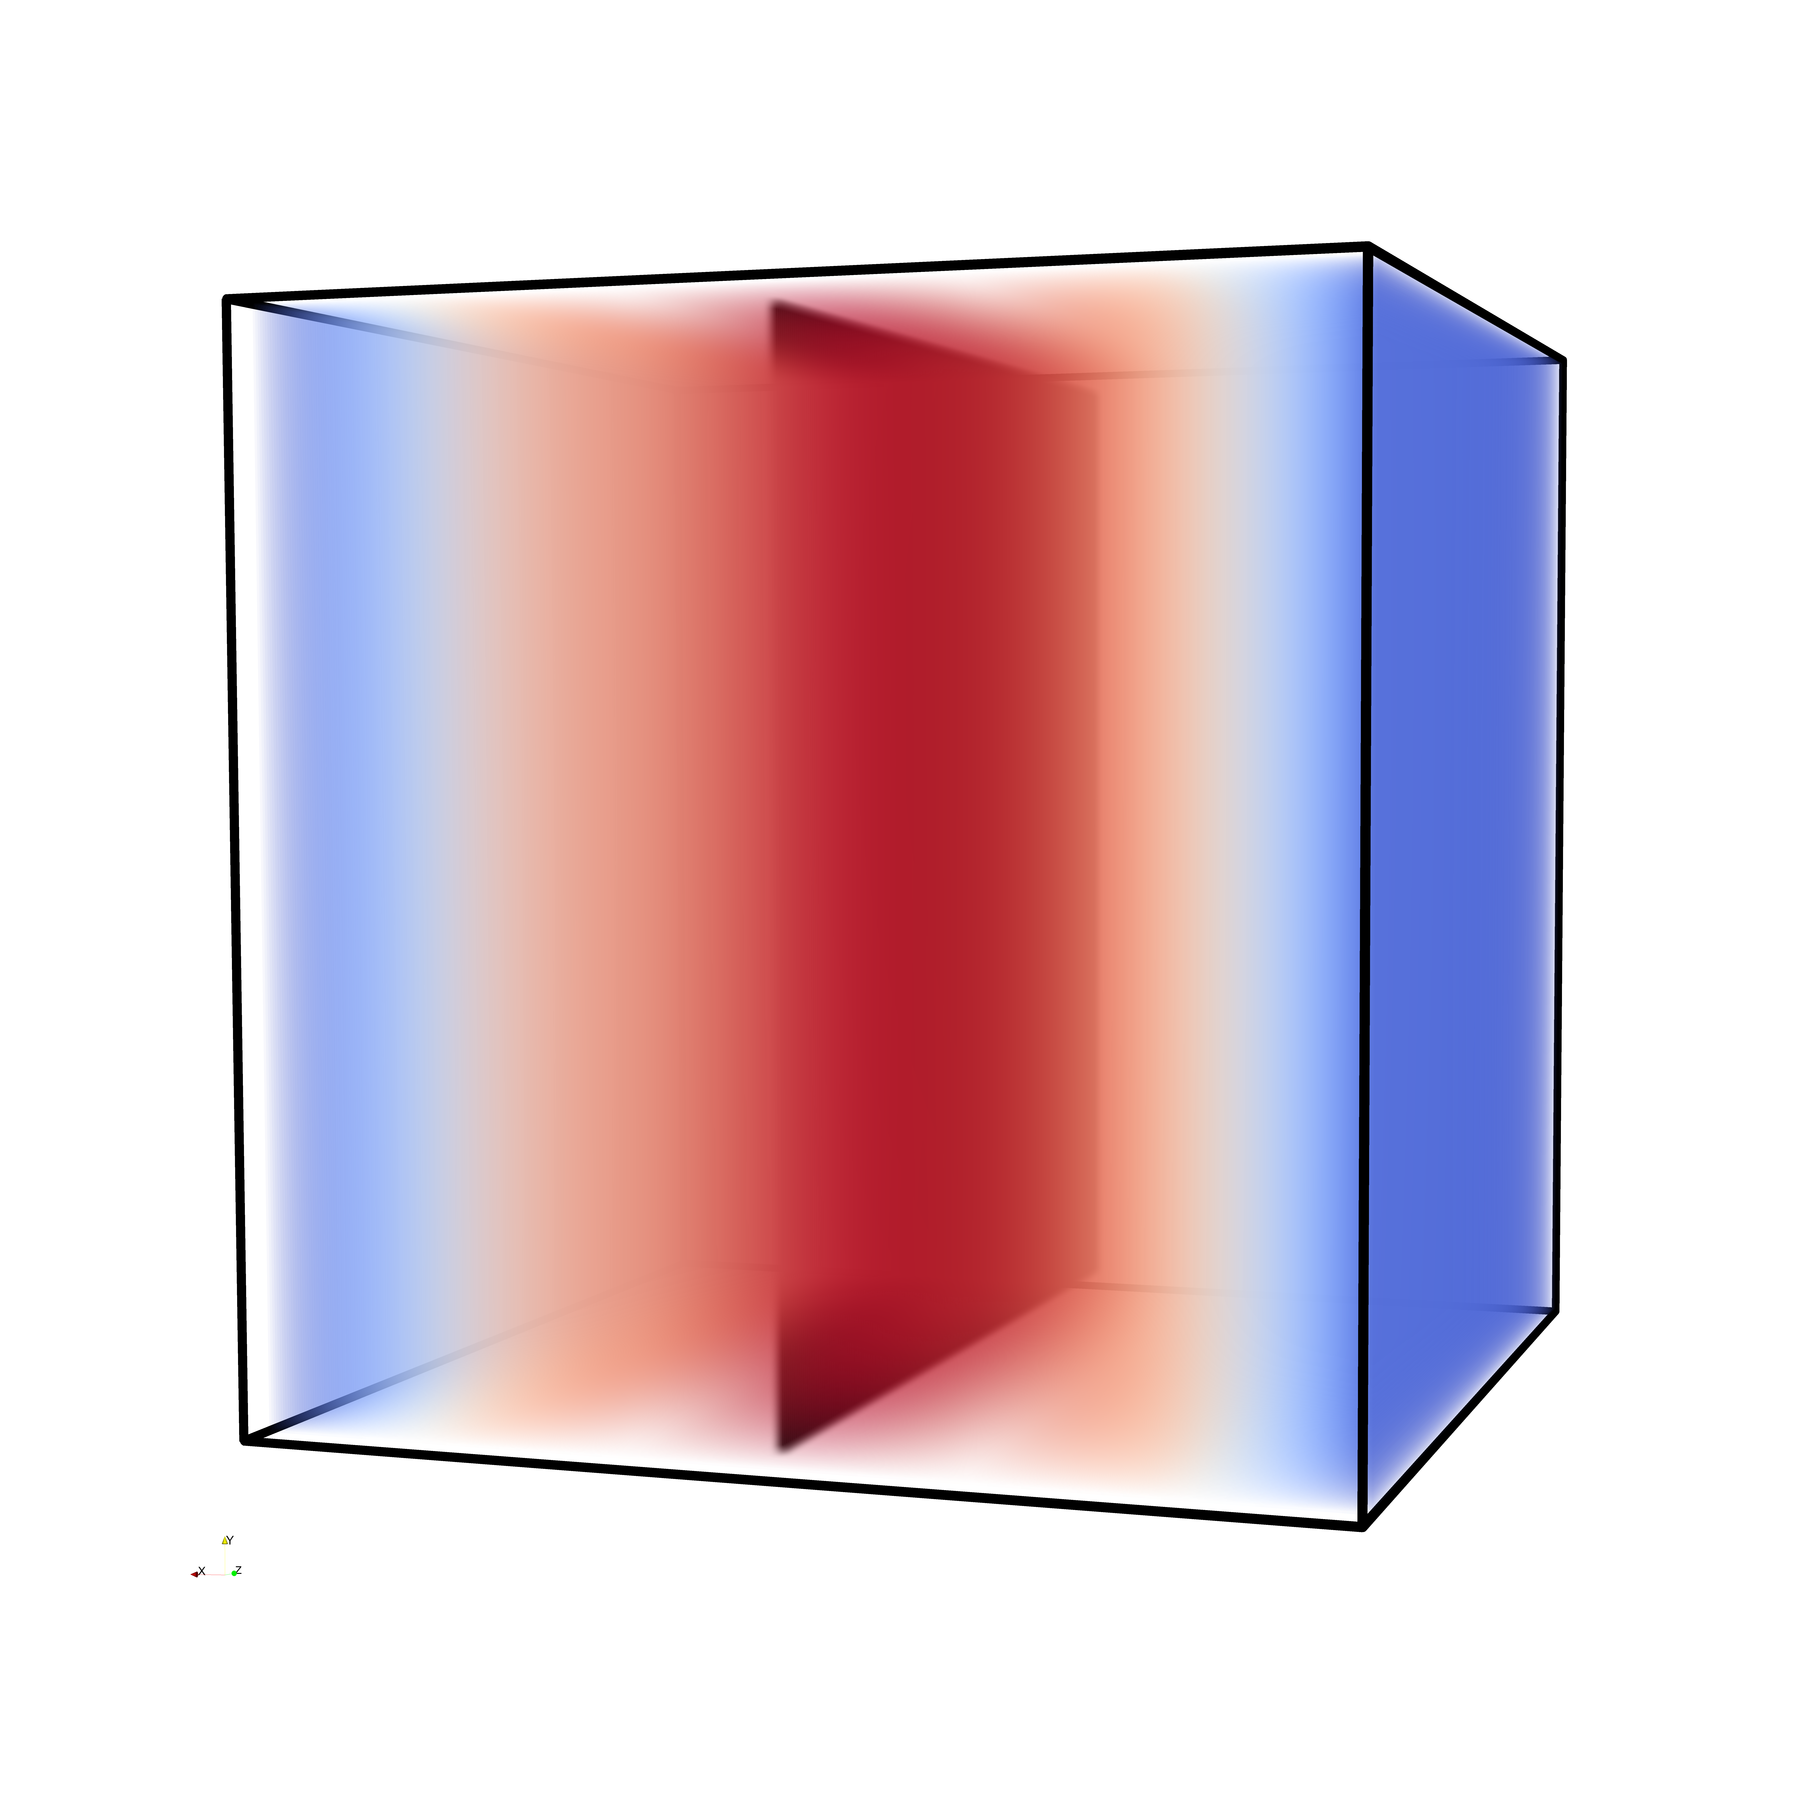
\includegraphics[width=\textwidth]{Images/func3D.png}
    \caption{$f(x,y,z)= -x^2$}
    \label{fig:ridge3D}
  \end{subfigure}
  \caption{Ridges of co-dimension one for the function $f(x)=-x^2$ with
  increasing dimensionality.}
\end{figure}

%%%%%%%%%%%%%%%%%%%%%%%%%%%%%%%%%%%%%%%%%%%%%%%%%%%%%%%%%%%%%%%%%%%%%%%%
\section{Marching Cubes}
%%%%%%%%%%%%%%%%%%%%%%%%%%%%%%%%%%%%%%%%%%%%%%%%%%%%%%%%%%%%%%%%%%%%%%%%

The Marching Cubes algorithm~\cite{MC} is a method to extract
isosurfaces from 3-dimensional discrete scalar fields. It got its name
due to the cell-wise extraction of the isosurface. The first step of the
algorithm is to check whether the nodes of the examined cell are either
below or above the desired isovalue. After that, a lookup table is
consulted that gives information on which edges of the cell connect such
two nodes. If every value is above or below the isovalue, the cell does
not contain a surface. Now linear interpolation is used to find the
location of the isosurface on the respective edges and the found points
are vertices of a triangle mesh. Figure~\ref{fig:MCTable} shows the
15 unique configurations for a surface in the cell, without
rotated variants. The same principle is used for the two dimensional
version, the Marching Squares algorithm. In that case the lookup table
is a lot simpler, as there are only four edges to check.

\begin{figure}
  \centering
  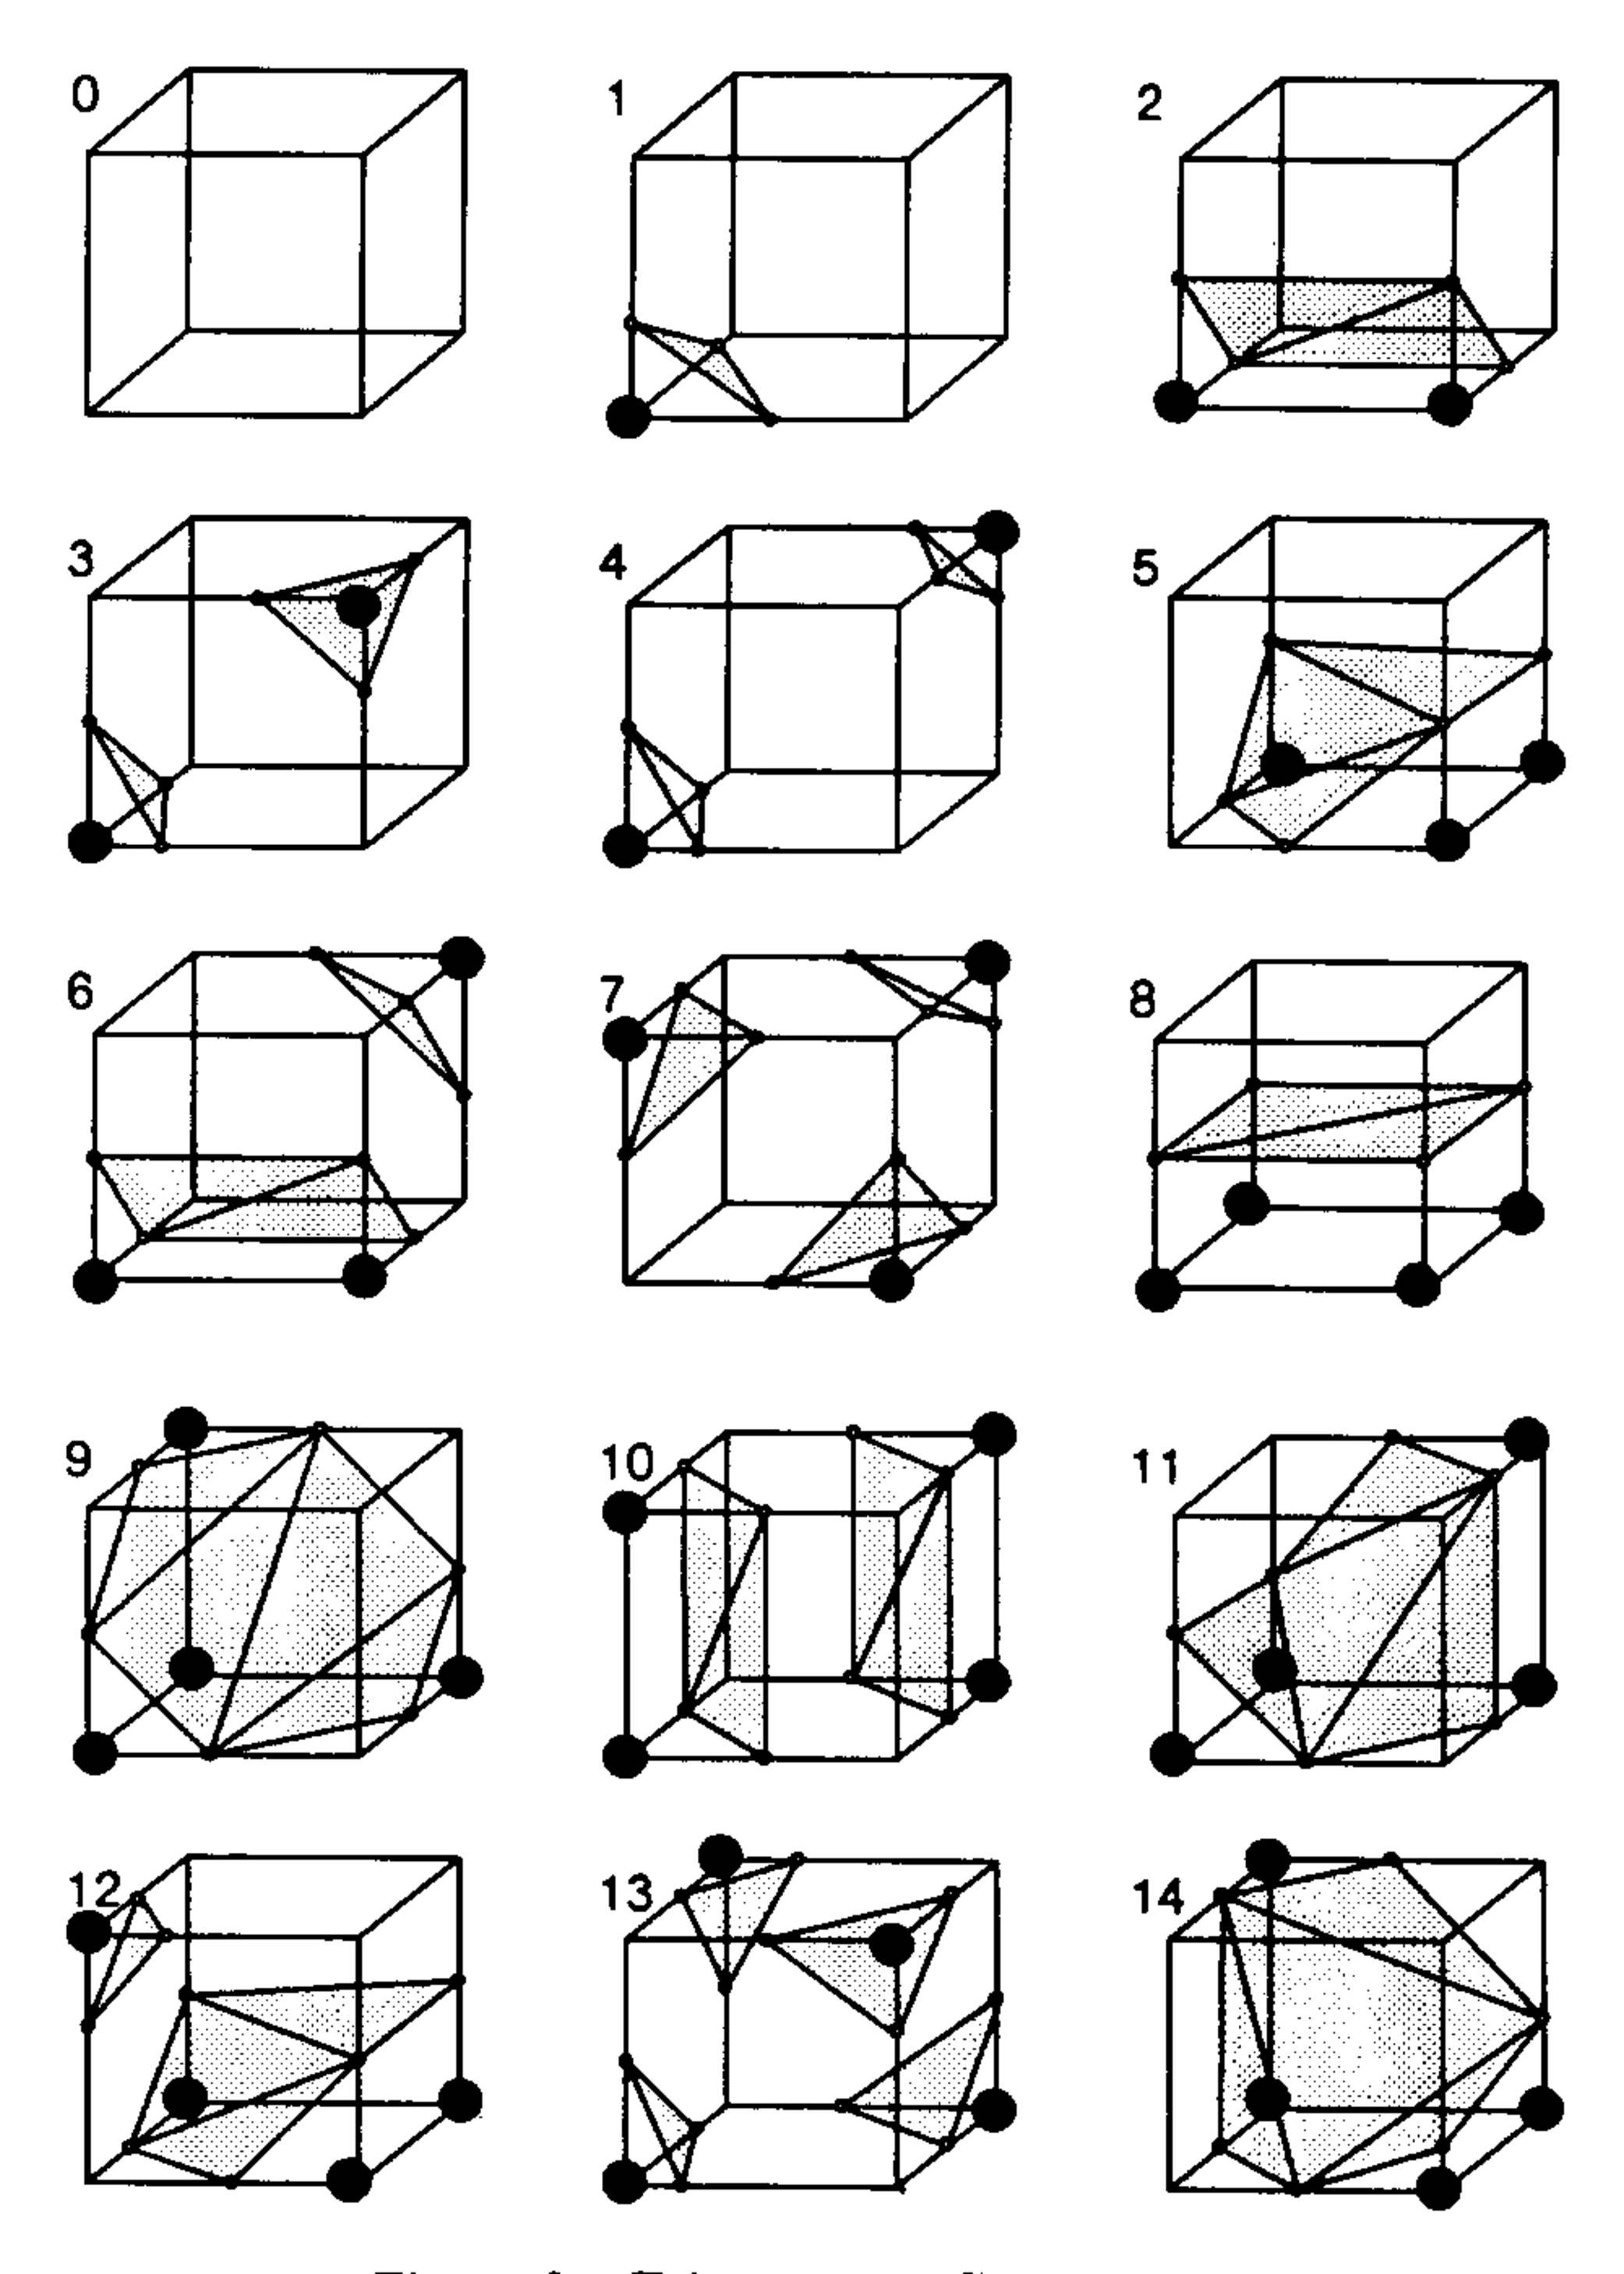
\includegraphics[width=0.6\textwidth]{Images/MCTable.pdf}
  \caption{Unique triangulations of the cubes according to Lorensen and
  Cline. Image from the original Marching Cubes publication~\cite{MC}.}
  \label{fig:MCTable}
\end{figure}

%%%%%%%%%%%%%%%%%%%%%%%%%%%%%%%%%%%%%%%%%%%%%%%%%%%%%%%%%%%%%%%%%%%%%%%%
\section{The Parallel Vectors Operator}\label{sec:PVO}
%%%%%%%%%%%%%%%%%%%%%%%%%%%%%%%%%%%%%%%%%%%%%%%%%%%%%%%%%%%%%%%%%%%%%%%%

When extracting ridge lines in three dimensions, one could check for the
conditions of Equation~\ref{eq:ridgeDot} and~\ref{eq:ridgeEV}. This
would require to extract two isolines simultaneously which is not
possible with the classical Marching Cubes algorithm. Another way would
be to check if the gradient $g$ is parallel to itself derived with the
Hessian, $g || H g$, as this implies that the gradient only changes
along its direction. Peikert and Roth proposed the Parallel Vectors
Operator~\cite{PV} as a versatile tool to find the set of points where
two vector fields are parallel. We will use their analytic solution for
triangular faces, and therefore every face of a cell is split into two
triangles. The vectors of the gradient field and their derivatives at
the nodes of an examined triangle can be expressed as a function of
local triangle coordinates $s$, $t$ and $u$ with $u$ set to $1$:
\begin{equation}
  g = V
  \begin{pmatrix}
    s\\
    t\\
    1
  \end{pmatrix}
\end{equation}
\begin{equation}
  H g = W
  \begin{pmatrix}
    s\\
    t\\
    1
  \end{pmatrix}.
\end{equation}
\noindent $V$ and $W$ are $3 \times 3$ matrices that are constructed
from the vectors $v_i$ and $w_i$ at the three nodes of the fields with:
\begin{align}
  &v_{12} = v_2 - v_1\\
  &v_{13} = v_3 - v_1\\
  &V = (v_1, v_{12}, v_{13})
\end{align}
\noindent and respectively for $w_i$ and $W$. Now two fields are
parallel when:

\begin{equation}
  V
  \begin{pmatrix}
    s\\
    t\\
    1
  \end{pmatrix}
  = \bar{\lambda} W
  \begin{pmatrix}
    s\\
    t\\
    1
  \end{pmatrix}
\end{equation}

\noindent If either $V$ or $W$ is invertible, ergo $\det{(V)}\neq 0 \vee
\det{(W)}\neq 0$ we can adjust the equation to get an eigenvector
problem:

\begin{equation}
  W^{-1} V
  \begin{pmatrix}
    s\\
    t\\
    1
  \end{pmatrix}
  = \bar{\lambda}
  \begin{pmatrix}
    s\\
    t\\
    1
  \end{pmatrix}
\end{equation}

\noindent Usually the matrix with the larger determinant is being
inverted. Now we can calculate the eigenvectors for the matrix $W^{-1}
V$ and scale them such that their last component is $1$. This provides
us with the local triangle coordinates $s$ and $t$ where the two fields
are parallel. If $s+t \leq 1$ and $s$ and $t$ are both greather than
zero, the point lies within the triangle and an extremum is found. With
the triangle coordinates the Hessian at the point can be interpolated to
check for $\lambda_2 < 0$ in the case of ridges or $\lambda_2 > 0$ for
valleys. Alternatively the minor or major eigenvectors of the Hessian
can be tested for parallelity, depending on the desired feature.
